\documentclass[twoside,spanish,a4paper,12pt]{tfg}
% Fuente: la clase solo cargaba inputenc (codificacion OT1 antigua), lo que hacia
% que acentos y enes se vieran "raros". Latin Modern + T1 da una tipografia limpia
% y escalable. No altera portada ni estructura.
\usepackage[T1]{fontenc}
\usepackage{lmodern}
\setlength{\emergencystretch}{2em}
\hbadness=10000
\vbadness=10000

% Colocación de flotantes. Los parámetros por defecto de LaTeX son muy
% restrictivos (bottomfraction 0.3, textfraction 0.2): una figura a ancho
% completo no cabe al pie y se ve empujada siempre a la cabecera, lo que parte
% los párrafos que cruzan el salto de página. Se relajan para que las figuras
% puedan ir también al pie o a una página propia, distribuyéndose mejor.
% Las figuras y tablas usan [tbp] (cabecera, pie o página propia) para no
% aterrizar a media página partiendo una frase; las excepciones puntuales
% llevan [ht] o [b] cuando su anclaje natural (frontera de sección, cita a
% una ecuación inmediatamente anterior) lo exige.
\renewcommand{\topfraction}{0.90}
\renewcommand{\bottomfraction}{0.80}
\renewcommand{\textfraction}{0.07}
\renewcommand{\floatpagefraction}{0.70}
\setcounter{topnumber}{3}
\setcounter{bottomnumber}{2}
\setcounter{totalnumber}{5}
\newcommand{\varname}[1]{\path{#1}}
% Permite usar flechas TikZ (<->, ->) con los caracteres activos de babel-spanish
\usetikzlibrary{babel}
\usepackage{multirow}
\usepackage{booktabs}
\usepackage{tabularx}

% El tutor pide "Tabla" en lugar del "Cuadro" por defecto de babel-spanish.
% Se aplica al inicio del documento para que no lo sobrescriba \captionsspanish.
% Se renombra también el título del índice de tablas (por defecto "Índice de
% cuadros") para que coincida con los pies ("Tabla") y con la entrada del TOC.
\AtBeginDocument{%
  \renewcommand{\tablename}{Tabla}%
  \renewcommand{\listtablename}{Índice de tablas}%
}

% Las páginas de relleno que inserta \cleardoublepage (versos en blanco al
% cerrar un capítulo en página impar) heredaban la cabecera "Capítulo N" o
% "Apéndices". Se redefine para que esos blancos no lleven cabecera ni pie.
\makeatletter
\renewcommand*{\cleardoublepage}{\clearpage\if@twoside
  \ifodd\c@page\else\hbox{}\thispagestyle{empty}\newpage
  \if@twocolumn\hbox{}\newpage\fi\fi\fi}
\makeatother

% Cabecera propia para la bibliografía: las páginas de referencias no son
% apéndices, así que no deben llevar la cabecera "Apéndices".
\fancypagestyle{bibliografia}{%
  \fancyhf{}%
  \fancyhead[EL,OR]{Bibliografía}%
  \fancyhead[OL,ER]{Página \thepage}%
  \renewcommand{\headrulewidth}{1pt}%
  \fancyfoot{}%
}

% Editar la titulación
\titulacion{Grado en Ciencia de Datos}

% Editar el título
\title{Desarrollo y evaluación de un método cuántico de selección de características}

% Si es una alumna se debe usar
% \authorlabel{Autora}
\authorlabel{Autor}
% Editar el nombre
\author{Carlos Gómez Sáez}


% Si hay varios tutores:
% \tutorlabel{Tutores}
% \tutor{Nombre del tutor 1 \\[2mm] Nombre del turor2}
% Si el tutor es masculino:
% \tutorlabel{Tutor}
\tutorlabel{Tutores}
\tutor{Yolanda Vives Gilabert \\[2mm] José D. Martín Guerrero}

% Editar: Poner mes y año de la convocatoria de lectura del TFM
\convocatoria{Julio 2026}

\begin{document}

% NO QUITAR ESTOS ELEMENTOS
\portada{}
\cleardoublepage{}

% Declaración sobre el uso de IA (recomendada por la UV en la convocatoria actual).
% Carlos: revisa este texto y ajústalo al modelo oficial de la UV y a tu uso real.
\thispagestyle{empty}
\vspace*{1\baselineskip}
\noindent{\large\bfseries Declaración sobre el uso de inteligencia artificial}
\vspace{0.5\baselineskip}

\noindent Durante el desarrollo de este Trabajo de Fin de Grado se han
utilizado herramientas de inteligencia artificial generativa como apoyo
en tareas de programación, depuración, organización documental, revisión
de estilo, traducción y mejora de la redacción. Estas herramientas se
han empleado como instrumento auxiliar bajo instrucciones, revisión y
criterio del autor.

\noindent El uso de estas herramientas no sustituye la autoría del
trabajo. El autor ha definido las decisiones metodológicas, ha
seleccionado los resultados, ha interpretado las evidencias y ha
elaborado, corregido y validado la redacción final de la memoria. Las
tablas, figuras, métricas y conclusiones presentadas proceden de los
datos, los \textit{scripts} y los archivos de evidencia generados por el
\textit{pipeline} reproducible descrito en la memoria, y no de salidas no
verificadas de sistemas de inteligencia artificial. En ningún caso se han
empleado estas herramientas para fabricar datos, resultados o
referencias, y el autor asume la plena responsabilidad sobre el contenido
del trabajo.
\cleardoublepage{}

\contraportada{}
\cleardoublepage{}
\declaracion{}
\cleardoublepage{}


% Editar: Resumen en Español (obligatorio)
\begin{resumen}
  La selección de características es una etapa central de la Ciencia de
  Datos: condiciona el rendimiento, la estabilidad y la interpretabilidad
  de los modelos supervisados. Este trabajo estudia la viabilidad de un
  método cuántico de selección de características (QFS, \textit{Quantum
  Feature Selection}) que formula el problema como una función binaria de
  relevancia y redundancia y lo resuelve mediante una simulación de
  átomos neutros con bloqueo de Rydberg. Para que la evaluación de ese
  método sea defendible, se construye primero una referencia clásica
  amplia y contrastada que no actúa solo como un baseline de rendimiento,
  sino como un sistema de coordenadas de relevancia, redundancia,
  estabilidad y coste sobre el que situar el método cuántico. La
  aportación principal no es un ranking de métodos, sino un diagnóstico:
  la referencia clásica, junto con el óptimo exacto del problema de
  optimización binaria subyacente, permite distinguir cuándo un eventual
  deterioro del método cuántico procede del criterio de selección y
  cuándo del proceso de optimización. En los conjuntos evaluados, QFS no
  aventaja de forma general a la selección de características clásica, pero
  el control exacto de la formulación QUBO permite atribuir sus
  deterioros a mecanismos distintos según el régimen del dato. Los
  resultados se interpretan con cautela y se circunscriben a los conjuntos
  de datos y al protocolo evaluados. El repositorio de entrega del trabajo
  está disponible en
  \url{https://github.com/gosacarpersonal/TFG---Desarrollo-y-Evaluacion-de-un-Metodo-Cuantico-de-Seleccion-de-Caracteristicas}.
\end{resumen}
\cleardoublepage{}

% Editar: Resumen en Inglés
\begin{abstract}
  Feature selection is a central Data Science task: it determines the
  performance, stability and interpretability of supervised models. This
  work studies the feasibility of a quantum feature selection method
  (QFS, \textit{Quantum Feature Selection}) that casts the problem as a
  binary relevance and redundancy objective and solves it through a
  neutral-atom simulation based on the Rydberg blockade. To make the
  evaluation of that method defensible, a broad and audited classical
  reference is built first; it acts not only as a performance baseline
  but as a coordinate system of relevance, redundancy, stability and cost
  on which to place the quantum method. The main contribution is not a
  ranking of methods, but a diagnosis: the classical reference, together
  with the exact optimum of the underlying binary optimization problem,
  makes it possible to tell whether any deterioration of the quantum
  method stems from the selection criterion or from the optimization
  process. Results are interpreted with caution and are restricted to the
  datasets and the protocol that were evaluated. The final submission
  repository is available at
  \url{https://github.com/gosacarpersonal/TFG---Desarrollo-y-Evaluacion-de-un-Metodo-Cuantico-de-Seleccion-de-Caracteristicas}.
\end{abstract}
\cleardoublepage{}

% Editar: Resumen en Valenciano
\begin{resum}
  \shorthandoff{'}%
  La selecció de característiques és una etapa central de la Ciència de
  Dades: condiciona el rendiment, l'estabilitat i la interpretabilitat
  dels models supervisats. Aquest treball estudia la viabilitat d'un
  mètode quàntic de selecció de característiques (QFS, \textit{Quantum
  Feature Selection}) que formula el problema com una funció binària de
  rellevància i redundància i el resol mitjançant una simulació d'àtoms
  neutres amb bloqueig de Rydberg. Perquè l'avaluació d'aquest mètode
  siga defensable, es construeix primer una referència clàssica àmplia i
  contrastada que no actua només com un baseline de rendiment, sinó com un
  sistema de coordenades de rellevància, redundància, estabilitat i cost
  sobre el qual situar el mètode quàntic. L'aportació principal no és un
  rànquing de mètodes, sinó un diagnòstic: la referència clàssica,
  juntament amb l'òptim exacte del problema d'optimització binària
  subjacent, permet distingir quan un eventual deteriorament del mètode
  quàntic prové del criteri de selecció i quan del procés d'optimització.
  Els resultats s'interpreten amb cautela i es limiten als conjunts de
  dades i al protocol avaluats. El repositori de lliurament del treball
  està disponible en
  \url{https://github.com/gosacarpersonal/TFG---Desarrollo-y-Evaluacion-de-un-Metodo-Cuantico-de-Seleccion-de-Caracteristicas}.
\end{resum}
\cleardoublepage{}


% Editar: Agradecimientos (opcional)
\begin{agradecimientos}
\end{agradecimientos}
\cleardoublepage{}

\tableofcontents

\cleardoublepage{}
\addcontentsline{toc}{chapter}{Índice de figuras}
\listoffigures

\cleardoublepage{}
\addcontentsline{toc}{chapter}{Índice de tablas}
\listoftables

\pagestyle{tfg}
\justify{}

\chapter{Introducción}
% Capítulo 1: Introducción, motivación y objetivos.

Este primer capítulo sitúa el problema de la selección de
características en el contexto de la Ciencia de Datos y delimita el
propósito del trabajo. En primer lugar se expone la motivación, que
conecta la reducción de dimensionalidad con la estabilidad, la
interpretabilidad y la validez de los modelos supervisados. A
continuación se fijan el objetivo general y los objetivos específicos
que guían el estudio.

\section{Motivación}

La selección de características es una de las etapas centrales del
aprendizaje automático supervisado. Su objetivo es identificar el
subconjunto de variables que conserva la capacidad predictiva del
problema reduciendo dimensionalidad, redundancia y coste
computacional~\cite{guyon2003}. En espacios de alta dimensionalidad,
una buena selección no es solo una optimización: condiciona la
estabilidad de los modelos, su interpretabilidad y la propia validez
de las conclusiones, como puso de manifiesto el desafío de selección
de características de NIPS~2003, un banco de referencia clásico para
problemas de alta dimensionalidad~\cite{guyon2004}.

El problema de seleccionar el mejor subconjunto de $k$ variables entre
$p$ candidatas es combinatorio y, en general, intratable de forma
exacta. Los métodos clásicos lo abordan mediante heurísticas: filtros
univariantes, métodos basados en regularización, importancias de
modelos de conjunto o criterios de relevancia--redundancia como
mRMR (\textit{minimum Redundancy Maximum Relevance})~\cite{peng2005}. En paralelo, la computación cuántica ofrece una
vía alternativa: formular la selección como un problema de
optimización binaria cuadrática sin restricciones (QUBO,
\textit{Quadratic Unconstrained Binary Optimization}) que combine
relevancia y redundancia en una única función objetivo, y resolverlo
sobre hardware cuántico~\cite{mucke2023}. En particular, las plataformas de átomos
neutros permiten codificar este tipo de problemas aprovechando el
fenómeno del bloqueo de Rydberg, que impide la excitación simultánea
de átomos vecinos y actúa de forma natural como una restricción de
exclusión entre variables redundantes~\cite{henriet2020}.

Este Trabajo de Fin de Grado analiza la viabilidad de un método
cuántico de selección de características (QFS, \textit{Quantum Feature
Selection}) basado en dicho fenómeno. El atractivo de esta vía es
computacional: QFS asigna un átomo (un cúbit) a cada variable
candidata y resuelve el compromiso relevancia--redundancia de forma
global sobre el hardware, de modo que un dispositivo de $n$ átomos puede
seleccionar características sobre un espacio de hasta $n$ variables en un
tiempo de ejecución muy corto, frente al coste combinatorio de la
búsqueda exacta clásica. Evaluar esa viabilidad de forma interpretable
exige caracterizar primero cada conjunto de datos: dónde reside la señal
predictiva, cómo se distribuye la redundancia, qué dimensionalidad
efectiva tiene y si las particiones permiten atribuir los resultados al
método y no al azar o a fugas de información. Con ese fin se construye
una referencia clásica que aporta, además de un baseline de rendimiento,
un sistema de coordenadas de relevancia, redundancia, estabilidad y coste
sobre el que situar el método cuántico.

De ahí la tesis que guía la memoria: el bloque clásico no es un mero
punto de comparación, sino el instrumento que permite leer el método
cuántico. Una caracterización clásica rigurosa anticipa qué componente
de QFS puede fallar en cada régimen de datos; y el contraste con el
óptimo exacto del problema de optimización subyacente permite, cuando
aparece un deterioro, separar si procede del criterio de información
mutua o del optimizador analógico que intenta alcanzarlo.

\section{Objetivos}

El objetivo general del TFG es analizar la viabilidad de un método de
selección de características que hace uso del bloqueo de Rydberg,
presente en tecnologías de átomos neutros, dentro de un protocolo
supervisado de Ciencia de Datos. La pregunta no es solo si QFS mejora
una métrica final, sino si puede competir con referencias clásicas
contrastadas y si sus resultados pueden atribuirse al criterio de
selección o al proceso de optimización. La propuesta del trabajo lo
desarrolla en seis objetivos específicos:

\begin{enumerate}
\item Revisar métodos clásicos de selección de características
  ampliamente utilizados y representativos de distintas familias de
  selección.
\item Seleccionar conjuntos de datos de referencia, diversos en número
  de muestras, dimensionalidad y tipo de variables, sobre los que
  evaluar los métodos de selección.
\item Realizar un estudio comparativo del rendimiento de los métodos
  clásicos sobre los conjuntos seleccionados.
\item Implementar y evaluar un método cuántico de selección de
  características basado en el bloqueo de Rydberg, conservando el núcleo
  de la formulación de referencia e incorporando adaptaciones operativas
  propias: un parámetro de separación $\beta$, una envolvente híbrida de
  preselección y la extensión del banco de pruebas a problemas
  multiclase y de alta dimensionalidad.
\item Comparar el rendimiento del método cuántico frente a los mejores
  selectores clásicos identificados, bajo un protocolo de evaluación
  común.
\item Analizar, mediante el óptimo exacto de la formulación QUBO, si las
  diferencias observadas entre el método cuántico y las referencias
  clásicas proceden del criterio de selección o del proceso de
  optimización analógica.
\end{enumerate}

El estudio clásico (objetivos 1--3) no se limita a ejecutar selectores:
se construye sobre datos validados, particiones sin fuga de información y
contrastes estadísticos explícitos, y mide propiedades que el rendimiento
no captura, como la estabilidad, la redundancia interna, la separación
frente al azar y la coherencia con las variables que usa el modelo. Sobre
esa base, los objetivos 4 a 6 implementan y evalúan el método cuántico
(su formulación, su codificación física y su contrato de evaluación), lo
comparan con los mejores selectores clásicos bajo el mismo protocolo y
añaden un control frente al óptimo exacto de la función de coste que
permite separar la calidad del criterio de la del optimizador. La
evaluación del método cuántico se realiza en un entorno simulado y bajo
una envolvente operativa controlada, por lo que las conclusiones se
refieren al protocolo experimental evaluado y no a una demostración en
hardware físico.



\chapter{Marco teórico}
% Capítulo 2: Marco teórico.

Este capítulo reúne los fundamentos necesarios para seguir el resto de
la memoria. Se parte de la selección de características y de su
formulación combinatoria como problema de optimización, y se introducen
después la computación cuántica adiabática y el bloqueo de Rydberg en
plataformas de átomos neutros, que sostienen el método cuántico
evaluado. Una sección adicional describe las herramientas de validación
estadística empleadas para distinguir resultados sólidos de relaciones
espurias. El capítulo termina relacionando estos fundamentos con las
decisiones concretas del trabajo.

\section{Selección de características}
\label{sec:mt-fs}

En aprendizaje automático supervisado, la selección de características
consiste en identificar el subconjunto de variables predictoras que
conserva la capacidad predictiva del problema reduciendo
dimensionalidad, redundancia y coste computacional~\cite{guyon2003}.
Sus beneficios habituales son tres: modelos más simples y más
interpretables, menor riesgo de sobreajuste cuando el número de
variables es alto en relación con el de muestras, y menor coste de
entrenamiento e inferencia. En espacios de alta dimensionalidad estos
beneficios dejan de ser una optimización y pasan a condicionar la
validez de las conclusiones, porque una parte de la señal aparente
puede deberse al azar de los contrastes múltiples.

Los métodos de selección se agrupan habitualmente en tres
familias~\cite{guyon2003}. Los métodos \emph{filter} puntúan cada
variable (o subconjunto) con un criterio estadístico independiente del
modelo, como los contrastes univariantes o la información mutua. Los
métodos \emph{wrapper} evalúan subconjuntos entrenando repetidamente un
modelo y midiendo su rendimiento. Los métodos \emph{embedded} obtienen la
selección como subproducto del propio entrenamiento, como ocurre con la
regularización $\ell_1$ o con las importancias de los modelos de
conjunto. Dentro de los filtros conviene distinguir además los criterios
\emph{supervisados}, que miran el target (contrastes univariantes,
información mutua), de los \emph{no supervisados}, que no lo usan. La
varianza es el ejemplo más simple de filtro no supervisado: puntúa cada
variable por su dispersión, sin mirar la etiqueta. En este trabajo se
incluye precisamente con ese papel, como control sin target frente al
resto de selectores supervisados~\cite{solorio2020}.

Una pieza central de muchos criterios de selección es la información
mutua~\cite{cover2006}. Para una variable $X$ y un target $Y$, la
información mutua $I(X;Y)$ mide la dependencia estadística entre
ambas, lineal o no lineal, y se anula únicamente cuando son
independientes:
\begin{equation}
  \label{eq:mi}
  I(X;Y) = \sum_{x \in X} \sum_{y \in Y} p(x,y)\,
  \log\frac{p(x,y)}{p(x)\,p(y)},
\end{equation}
donde $p(x,y)$ es la distribución conjunta de $X$ e $Y$, y $p(x)$ y
$p(y)$ sus distribuciones marginales. Esta generalidad la hace adecuada
tanto para medir la
\emph{relevancia} de una variable respecto al target como la
\emph{redundancia} entre pares de variables. Seleccionar solo por
relevancia tiende a producir subconjuntos redundantes, donde varias
variables aportan información solapada; el criterio mRMR
(\textit{minimum Redundancy Maximum Relevance})~\cite{peng2005}
formaliza el compromiso entre ambas cantidades y lo resuelve de forma
voraz, añadiendo en cada paso la variable que maximiza la relevancia
penalizada por la redundancia con las ya elegidas.

\section{Formulación combinatoria del problema}
\label{sec:mt-qubo}

Elegir el mejor subconjunto de $k$ variables entre $p$ candidatas es
un problema combinatorio: el número de subconjuntos crece
exponencialmente y la búsqueda exacta resulta intratable salvo en
espacios muy pequeños. Esta es la razón de que los métodos clásicos
recurran a heurísticas voraces o a criterios univariantes que no
garantizan el óptimo global.

El compromiso relevancia--redundancia admite una formulación exacta
como problema de optimización binaria cuadrática sin restricciones
(QUBO). Esta es la formulación que Mücke et al.~\cite{mucke2023}
proponen para la selección de características y que el método cuántico
evaluado en este trabajo adopta: cada variable se representa con una
incógnita binaria $x_i \in \{0,1\}$ que indica si entra en el
subconjunto, el término lineal premia la relevancia individual y el
término cuadrático penaliza la selección simultánea de pares
redundantes, ponderados por un parámetro $\alpha \in [0,1]$:
\begin{equation}
  \label{eq:qubo}
  Q(x;\alpha) = -\alpha \sum_{i} I_i\, x_i
  + (1-\alpha) \sum_{i<j} R_{ij}\, x_i x_j,
\end{equation}
donde $I_i$ es la relevancia de la variable $i$ con el target y $R_{ij}$
la redundancia entre las variables $i$ y $j$. Minimizar $Q$ premia
seleccionar variables relevantes (término lineal negativo) y penaliza
incluir pares redundantes (término cuadrático positivo).

Una propiedad de esta formulación resulta central para todo el
trabajo: el parámetro $\alpha$ no es solo un balance, sino que induce
una trayectoria discreta de soluciones al variar el compromiso entre
relevancia y redundancia. En las instancias reales esa trayectoria es
monótona en la práctica, pero puede permanecer constante durante varios
valores de $\alpha$, saltar presupuestos y presentar empates. Conviene
adelantar aquí una distinción que el capítulo de métodos retoma: este
recorrido de $\alpha$ pertenece al \emph{control exacto} del criterio (el
óptimo del QUBO resuelto de forma exacta), que se usa como referencia;
la configuración operativa del método cuántico, en cambio, fija un único
valor de $\alpha$ y obtiene el presupuesto por otra vía. Cuando se
necesita comparar exactamente a un presupuesto $k$, ese control exacto
usa el recorrido de $\alpha$ como guía y resuelve además el QUBO con la
restricción explícita $\sum_i x_i=k$. El barrido de $\alpha$ se
interpreta, por tanto, como una escalera discreta de presupuestos
observados, no como una garantía de
pasos unitarios para cualquier matriz $I_i,R_{ij}$
(Figura~\ref{fig:escalera-alpha}).

\begin{figure}[!htbp]
  \centering
  
\includegraphics[width=0.82\textwidth]{mt_escalera_alpha.pdf}
  \caption[Trayectoria de $\alpha$ como escalera de presupuestos]{Esquema
    de la trayectoria de soluciones del QUBO al recorrer $\alpha$ de $0$ a
    $1$. La cardinalidad del óptimo $k=\sum_i x_i$ crece a saltos, con
    tramos planos en los que el presupuesto no cambia. Cuando la escalera
    salta un presupuesto de referencia $k^{\star}$ (línea roja), ese
    presupuesto se obtiene resolviendo el QUBO con la restricción explícita
    $\sum_i x_i = k^{\star}$. El esquema es ilustrativo; las trayectorias
    reales por dataset aparecen en el capítulo de resultados.}
  \label{fig:escalera-alpha}
\end{figure}

Esta clase de problemas conecta directamente con la teoría de grafos:
si las variables se ven como nodos ponderados por su relevancia y las
redundancias altas se transforman en aristas o interacciones de bloqueo,
seleccionar variables relevantes y mutuamente no redundantes se aproxima
al problema de buscar un conjunto independiente de peso máximo
(\textit{Maximum Weighted Independent Set}, MWIS)~\cite{arribas2025}.
El QUBO de la ecuación~\ref{eq:qubo} mantiene penalizaciones blandas,
mientras que el MWIS físico inducido por el bloqueo de Rydberg impone
exclusiones duras; el método cuántico evaluado se apoya precisamente en
esa correspondencia geométrica, no en una identidad algebraica sin
condiciones.

\section{Fundamentos de computación cuántica}
\label{sec:mt-fundamentos-cuantica}

Antes de presentar el paradigma adiabático y su realización física
conviene fijar los conceptos básicos sobre los que se construye la
aproximación cuántica de este trabajo (Figura~\ref{fig:cubit}).

\textbf{Estado cuántico y cúbit.} La unidad de información de la
computación cuántica es el \emph{cúbit} (bit cuántico): un sistema físico
de dos niveles cuyo estado se describe, en notación de Dirac, como un
vector $|\psi\rangle = \alpha\,|0\rangle + \beta\,|1\rangle$ en un espacio
de Hilbert de dimensión dos, con $\alpha,\beta\in\mathbb{C}$ y
$|\alpha|^2+|\beta|^2=1$. Los estados base $|0\rangle$ y $|1\rangle$ son el
análogo cuántico de los valores $0$ y $1$ de un bit clásico.

\textbf{Superposición.} A diferencia de un bit, que toma un único valor,
un cúbit puede encontrarse en una \emph{superposición} de ambos estados
base ($\alpha$ y $\beta$ no nulos a la vez). Al medirlo en la base
computacional se obtiene $0$ con probabilidad $|\alpha|^2$ y $1$ con
probabilidad $|\beta|^2$, y el estado colapsa al resultado observado. Un
registro de $n$ cúbits se describe en un espacio de Hilbert de dimensión
$2^n$, lo que permite codificar amplitudes asociadas a las $2^n$ cadenas
de bits posibles; la información finalmente accesible queda, no obstante,
limitada por la medición y por la dinámica concreta del algoritmo. Sobre
esa estructura se apoya el interés de la computación cuántica en
problemas de optimización combinatoria.

\textbf{Entrelazamiento.} Cuando el estado conjunto de dos o más cúbits no
puede escribirse como producto de los estados individuales, se dice que
están \emph{entrelazados}: sus medidas quedan correlacionadas de una forma
que no admite una explicación clásica local. El entrelazamiento es el
recurso que distingue a un sistema cuántico de una colección de bits
independientes y el que permite codificar interacciones entre variables.

\textbf{Hamiltoniano.} La energía de un sistema cuántico se describe
mediante un operador hermítico $H$ denominado \emph{hamiltoniano}, cuyos
autovalores son las energías accesibles del sistema y cuyos autovectores
son los estados estacionarios correspondientes; el autovector de menor
autovalor es el \emph{estado fundamental} (\textit{ground state}). El
hamiltoniano gobierna además la evolución temporal del estado a través de
la ecuación de Schrödinger. Su papel es central en este trabajo: la
estrategia cuántica empleada consiste en construir un hamiltoniano cuyo
estado fundamental codifique la solución del problema de optimización
(el subconjunto de características óptimo), de modo que hallar el
mínimo de energía equivale a resolver el problema. Las dos secciones
siguientes describen, respectivamente, cómo se alcanza ese estado
fundamental (computación adiabática) y cómo se realiza físicamente el
hamiltoniano mediante átomos neutros con bloqueo de Rydberg.

\begin{figure}[!htbp]
  \centering
  
\includegraphics[width=\textwidth]{mt_cubit_bloch.pdf}
  \caption[Conceptos básicos de computación cuántica]{Conceptos básicos
    sobre los que se construye la aproximación cuántica. (A) Un cúbit se
    representa como un punto en la esfera de Bloch; los polos son los
    estados base $|0\rangle$ y $|1\rangle$ y cualquier otro punto es una
    superposición $\alpha|0\rangle+\beta|1\rangle$. (B) Dos cúbits
    entrelazados comparten un estado conjunto que no puede factorizarse en
    estados individuales: medir uno condiciona la medida del otro. (C) El
    hamiltoniano fija las energías accesibles del sistema; su autovector
    de menor energía, el estado fundamental, es el que codifica la
    solución del problema.}
  \label{fig:cubit}
\end{figure}

\section{Computación cuántica adiabática}
\label{sec:mt-adiabatica}

Sobre esos fundamentos se construyen dos grandes paradigmas de
computación cuántica. El más conocido es el \emph{modelo de puertas}, que
transforma el estado de los cúbits aplicando una secuencia de operaciones
discretas, de forma análoga a las puertas lógicas de un circuito clásico.
Junto a él existe un paradigma analógico, especialmente adecuado para la
optimización combinatoria: la computación
adiabática~\cite{schuld2021, wittek2014}. La idea es preparar el
sistema en el estado fundamental de un hamiltoniano sencillo y
deformarlo de manera suficientemente lenta hacia un hamiltoniano final
cuyo estado de mínima energía codifica la solución del problema. De acuerdo con el
teorema adiabático, si la evolución es lenta en comparación con la
separación entre niveles de energía y se cumplen las condiciones del
modelo, el sistema tiende a permanecer en el estado fundamental durante
todo el proceso
(Figura~\ref{fig:adiabatica-esquema}).

\begin{figure}[!htbp]
  \centering
  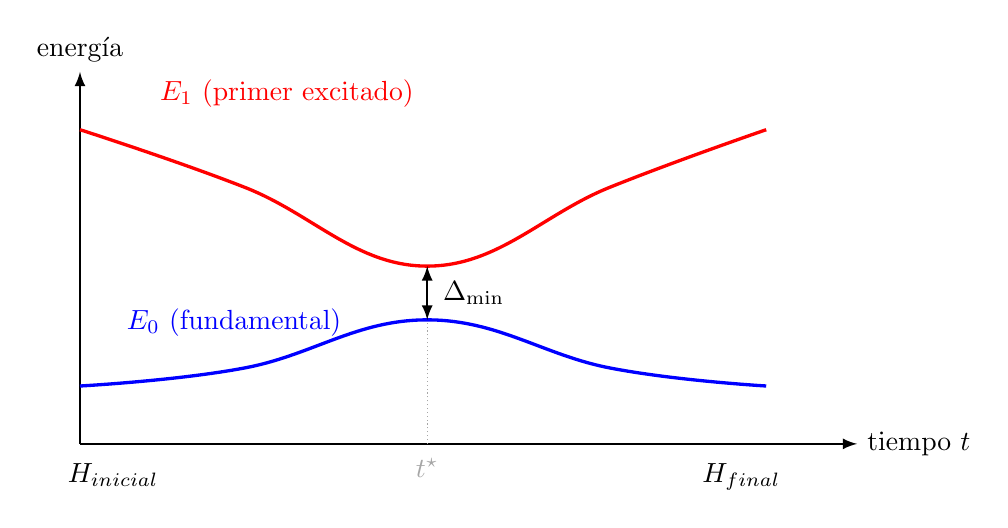
\begin{tikzpicture}[scale=1.05]
    % ejes
    \draw[-latex,thick] (0,0) -- (9.4,0) node[right] {tiempo $t$};
    \draw[-latex,thick] (0,0) -- (0,4.5) node[above] {energía};
    % linea vertical en el instante del gap minimo y region sombreada
    \draw[densely dotted,gray!70] (4.2,0) -- (4.2,2.15);
    \node[gray!70,anchor=north] at (4.2,-0.06) {$t^{\star}$};
    % curva del estado fundamental E0
    \draw[very thick,blue] plot[smooth,tension=0.7]
      coordinates {(0,0.7)(2,0.92)(4.2,1.5)(6.4,0.92)(8.3,0.7)};
    % curva del primer estado excitado E1
    \draw[very thick,red] plot[smooth,tension=0.7]
      coordinates {(0,3.8)(2,3.1)(4.2,2.15)(6.4,3.1)(8.3,3.8)};
    % gap minimo, claramente acotado
    \draw[latex-latex,thick] (4.2,1.5) -- (4.2,2.15) node[midway,right=2pt] {$\Delta_{\min}$};
    % etiquetas de las curvas, en bandas despejadas para no solapar las curvas
    \node[blue,anchor=south west] at (0.45,1.18) {$E_0$ (fundamental)};
    \node[red,anchor=south west] at (0.85,3.95) {$E_1$ (primer excitado)};
    % hamiltonianos inicial y final
    \node[anchor=north] at (0.4,-0.12) {$H_{\text{inicial}}$};
    \node[anchor=north] at (8.0,-0.12) {$H_{\text{final}}$};
  \end{tikzpicture}
  \caption[Esquema de la evolución adiabática]{Esquema de la evolución
    adiabática. El sistema parte del
    estado fundamental de un hamiltoniano sencillo $H_{\text{inicial}}$ y
    se deforma lentamente hacia $H_{\text{final}}$, cuyo fundamental
    codifica la solución. La separación entre el nivel fundamental $E_0$ y
    el primer excitado $E_1$ alcanza un mínimo $\Delta_{\min}$; el teorema
    adiabático exige una evolución lenta frente a ese gap para no abandonar
    el estado fundamental.}
  \label{fig:adiabatica-esquema}
\end{figure}

El factor que gobierna esa exigencia es el gap mínimo $\Delta_{\min}$: la
condición adiabática pide un tiempo de evolución que crece, a grandes
rasgos, como $1/\Delta_{\min}^2$, de modo que las instancias con un gap
pequeño son las más difíciles de resolver sin abandonar el estado
fundamental. Por eso la calidad de la solución depende del diseño de los
\emph{drivings}: los perfiles temporales de los campos de control que
gobiernan la evolución. En el protocolo concreto que emplea el método
evaluado, esos campos son tres: la frecuencia de Rabi $\Omega(t)$, que
mide la intensidad con que el láser acopla los estados $|0\rangle$ y
$|1\rangle$ y, por tanto, la rapidez con que un átomo puede pasar de uno a
otro; el \textit{detuning} global $\Delta(t)$, el desfase entre la
frecuencia del láser de control y la de la transición atómica, que regula
cuántas excitaciones resultan energéticamente favorables; y un
\textit{detuning} local por átomo que codifica la relevancia de cada
variable. Los tres se programan en dos pasos para mantener la
adiabaticidad con tiempos finitos, un problema de control activo en la
literatura~\cite{ding2021, arribas2025}. Al final de
la evolución, la medición del sistema en la base computacional produce
cadenas binarias; repetir el proceso genera una distribución de
soluciones candidatas en la que las configuraciones de menor energía
aparecen con mayor probabilidad.

\section{Átomos neutros y bloqueo de Rydberg}
\label{sec:mt-rydberg}

Las plataformas de átomos neutros confinan átomos individuales
mediante pinzas ópticas, lo que permite disponerlos en geometrías
bidimensionales arbitrarias y reconfigurables~\cite{henriet2020}. Cada
átomo actúa como un cúbit: el estado fundamental representa el valor
0 y un estado de Rydberg altamente excitado representa el valor 1.
Dos átomos excitados simultáneamente a estados de Rydberg
interactúan con una intensidad que decae con la sexta potencia de la
distancia que los separa. Esta interacción, de tipo van der Waals, se
describe como
\begin{equation}
  \label{eq:vdw}
  V_{ij} = \frac{C_6}{r_{ij}^{6}},
\end{equation}
donde $r_{ij}$ es la distancia entre los átomos $i$ y $j$ y $C_6$ un
coeficiente que depende del estado de Rydberg empleado. La fuerte
dependencia con $r_{ij}^{-6}$ es la que hace que la interacción pase de
despreciable a dominante en un margen estrecho de distancias.

De esa interacción surge el fenómeno que explota este trabajo: el
\emph{bloqueo de Rydberg}. Cuando dos átomos están más cerca que una
distancia crítica, llamada radio de bloqueo, la interacción desplaza
tanto la energía del estado doblemente excitado que el láser de
control no puede poblarlo: dentro de un volumen de bloqueo solo cabe
una excitación. El hardware implementa así, de forma nativa, una
restricción dura de exclusión entre vecinos, que es exactamente la
restricción de independencia del MWIS (Figura~\ref{fig:rydberg-esquema}).
Esta correspondencia ha
permitido resolver experimentalmente instancias del conjunto
independiente máximo con cientos de átomos~\cite{ebadi2022} y es la
base del método de selección de características evaluado en este
trabajo~\cite{orquin2026}.

\begin{figure}[!htbp]
  \centering
  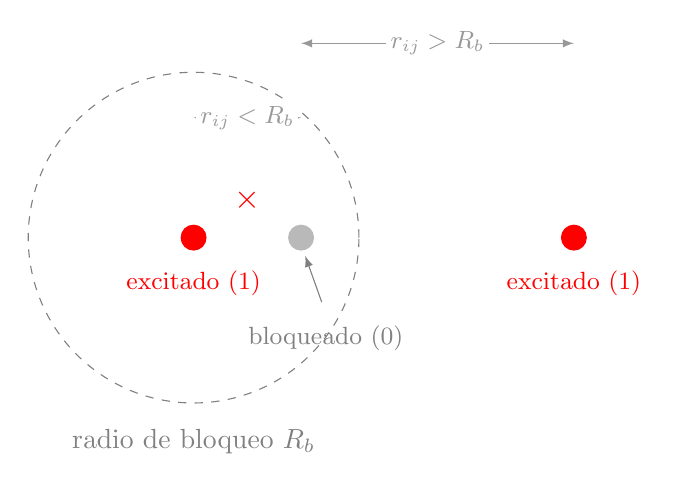
\begin{tikzpicture}[scale=1.05]
    % radio de bloqueo alrededor del atomo excitado izquierdo
    \draw[dashed,gray] (0,0) circle (2.0);
    \node[gray,anchor=north] at (0,-2.2) {radio de bloqueo $R_b$};
    % distancias, arriba y con fondo blanco para no solaparse con nada
    \draw[latex-latex,gray!80] (0,1.45) -- (1.3,1.45)
      node[midway,fill=white,inner sep=1.5pt] {\small $r_{ij}<R_b$};
    \draw[latex-latex,gray!80] (1.3,2.35) -- (4.6,2.35)
      node[midway,fill=white,inner sep=1.5pt] {\small $r_{ij}>R_b$};
    % atomo excitado (1) izquierdo, etiqueta debajo
    \filldraw[red] (0,0) circle (0.15);
    \node[red,anchor=north] at (0,-0.28) {\small excitado ($1$)};
    % atomo vecino dentro del radio -> bloqueado, etiqueta debajo y separada
    \filldraw[gray!55] (1.3,0) circle (0.15);
    \node[gray,anchor=north] at (1.6,-0.95) {\small bloqueado ($0$)};
    \draw[gray,-latex] (1.55,-0.78) -- (1.35,-0.22);
    % cruz de prohibicion entre los dos vecinos
    \node[red] at (0.65,0.45) {\large$\times$};
    % atomo lejano fuera del radio -> puede excitarse
    \filldraw[red] (4.6,0) circle (0.15);
    \node[red,anchor=north] at (4.6,-0.28) {\small excitado ($1$)};
  \end{tikzpicture}
  \caption[Bloqueo de Rydberg]{Bloqueo de Rydberg. Dos átomos dentro
    del radio de bloqueo
    $R_b$ no pueden excitarse a la vez: si uno ocupa el estado de Rydberg
    ($1$), el desplazamiento de energía de van der Waals
    (ecuación~\ref{eq:vdw}) impide poblar el de su vecino, que queda en el
    estado fundamental ($0$). Un átomo fuera de $R_b$ sí puede excitarse.
    Esta exclusión entre vecinos reproduce la restricción de
    independencia del MWIS sobre el grafo de características.}
  \label{fig:rydberg-esquema}
\end{figure}

\section{Herramientas de validación estadística}
\label{sec:mt-validacion}

Un estudio que examina muchas variables con muchos contrastes genera
asociaciones aparentes por puro azar: a un nivel de significación
fijo, la proporción esperada de falsos positivos crece con el número
de contrastes realizados. Este trabajo adopta cuatro salvaguardas
sistemáticas frente a ese riesgo, que se aplican en todas las fases
del bloque experimental: la corrección por multiplicidad sobre la
asociación variable--target, la comprobación de que el preprocesado y
el particionado no alteran el problema, y una cadena de contrastes que
autoriza el diagnóstico final.

Los contrastes empleados son no paramétricos para no depender de la
normalidad. La asociación de una variable numérica con un target de dos
grupos se contrasta con la prueba de rangos de Mann--Whitney~\cite{mann1947},
y con la de Kruskal--Wallis~\cite{kruskal1952} cuando el target tiene
más de dos clases; la asociación entre variables categóricas se contrasta
con la prueba $\chi^2$ de independencia. La monotonía entre dos
ordenaciones (por ejemplo, el ranking de relevancia antes y después del
preprocesado) se mide con la correlación de rangos de Spearman
$\rho\in[-1,1]$, que vale $1$ cuando ambas ordenaciones coinciden. Para
comparar la distribución de una misma variable entre dos particiones se
emplean tres medidas complementarias, todas nulas cuando las
distribuciones coinciden: el estadístico de Kolmogorov--Smirnov, que toma
la máxima distancia vertical entre las funciones de distribución
acumuladas y es sensible a desplazamientos locales; la distancia de
Wasserstein estandarizada, que cuantifica el «coste» de transformar una
distribución en la otra y capta diferencias globales de forma; y el
índice de estabilidad poblacional (PSI), un indicador de uso habitual en
la industria para detectar cambios de población entre dos muestras. El
desplazamiento de la proporción de clases del target entre particiones se
contrasta, además, con la prueba $\chi^2$ y, cuando las frecuencias son
pequeñas, con la prueba exacta de Fisher.

La primera es la corrección por comparaciones múltiples. Cuando se
contrasta una batería de variables contra el target, los p-valores se
ajustan con el procedimiento de Benjamini--Hochberg~\cite{benjamini1995}:
se ordenan los $m$ p-valores de menor a mayor y se rechaza la hipótesis
nula para el mayor $p_{(i)}$ que cumple $p_{(i)} \le \frac{i}{m}\,q$,
con lo que se controla en $q$ la proporción esperada de falsos
descubrimientos (FDR, \textit{False Discovery Rate}). Una variable solo
se considera asociada al target si su contraste sobrevive a esa
corrección, no si resulta significativa de forma aislada.

La segunda es la distinción entre significancia y magnitud. Un
p-valor responde si un resultado es compatible con el azar, no si es
relevante: con tamaños muestrales grandes, efectos minúsculos resultan
estadísticamente significativos. Por ello, cada contraste se acompaña de su tamaño de efecto, acotado y
comparable entre problemas: la delta de Cliff~\cite{cliff1993} para los
contrastes de dos grupos de Mann--Whitney~\cite{mann1947}, que mide en
$[-1,1]$ cuánto tiende un grupo a superar al otro; el épsilon cuadrado
para los de Kruskal--Wallis~\cite{kruskal1952}, que expresa en $[0,1]$
la fracción de variabilidad por rangos atribuible al grupo; y la V de
Cramér para los contrastes de independencia entre variables
categóricas, también en $[0,1]$. La lectura conjunta de significancia y
magnitud es la que sostiene las conclusiones.

La tercera es la construcción de distribuciones nulas empíricas por
permutación. Cuando la distribución nula de un estadístico no es
conocida, como ocurre con las puntuaciones de los selectores de
características, se genera empíricamente permutando el target y
recalculando la puntuación; un valor observado solo se considera señal
si supera el percentil alto de esa distribución nula. El mismo
principio se aplica al rendimiento de los modelos finales mediante la
permutación de etiquetas, que verifica que ningún resultado es
compatible con un clasificador aleatorio.

La cuarta es la cuantificación de la incertidumbre por remuestreo. Los
intervalos de confianza de las métricas de prueba se obtienen por
\textit{bootstrap}~\cite{efron1979} sobre las predicciones, sin
supuestos distribucionales, y las comparaciones entre configuraciones
se realizan de forma pareada sobre las mismas filas. Esta lógica de
contrastar lo observado frente a lo que el azar o el criterio regalan
se extiende a la fase cuántica: la comparación con el óptimo exacto de
la función de coste, descrita en el capítulo de métodos, permite
distinguir la calidad de la optimización de la calidad del criterio
optimizado.

% Estado del arte integrado como sección del marco teórico (antes era el
% Capítulo 3, demasiado corto como capítulo independiente).
\section{Estado del arte}
\label{sec:mt-estado-arte}

Esta sección revisa los trabajos previos sobre los que se apoya la
propuesta, organizados por familias de enfoques. Se examinan primero
los métodos clásicos de selección de características y, a continuación,
las líneas de optimización cuántica de problemas combinatorios y el uso
de átomos de Rydberg en tareas de optimización. La última subsección se
centra en las formulaciones cuánticas de la selección de
características, que constituyen el antecedente directo del método
estudiado.

\subsection{Métodos clásicos de selección de características}

Sobre las tres familias descritas en el marco teórico
(sección~\ref{sec:mt-fs}), la literatura ha consolidado un repertorio de
selectores que reaparecen de forma
recurrente como referencia. Entre los \emph{filter}, la puntuación F de ANOVA
y la información mutua son los criterios supervisados más utilizados por
su bajo coste, y la varianza se mantiene como criterio no supervisado de
control~\cite{solorio2020}. Entre los métodos \emph{embedded}, los más
extendidos son la regularización $\ell_1$ y las importancias por
impureza de los bosques aleatorios~\cite{breiman2001}, mientras que el
criterio mRMR~\cite{peng2005} sigue siendo la referencia para incorporar
la redundancia de forma explícita. Entre los \emph{wrapper}, el algoritmo
Boruta~\cite{kursa2010}, que compara la importancia de cada variable con
la de copias permutadas (variables \textit{sombra}) y retiene solo las
que la superan de forma consistente, se ha convertido en uno de los
puntos de comparación habituales en la literatura reciente de selección
cuántica, pese a que su coste crece con los reentrenos del modelo base.

Esa misma literatura ha señalado que el rendimiento predictivo no basta
para caracterizar un selector. La estabilidad de los subconjuntos ante
perturbaciones como el cambio de semilla o de muestra se cuantifica con
índices de solape corregidos por azar, como el de
Kuncheva~\cite{kuncheva2007}: un selector inestable produce subconjuntos
poco reproducibles aunque su rendimiento medio sea alto. La estabilidad
y la redundancia interna se han establecido así como dimensiones de
evaluación complementarias al rendimiento.

\subsection{Optimización cuántica de problemas combinatorios}

La resolución de problemas QUBO es una de las aplicaciones más
estudiadas de la computación cuántica actual~\cite{schuld2021,
wittek2014}. Se han explorado tres líneas principales: el
\textit{quantum annealing} o recocido cuántico, un hardware dedicado que
relaja lentamente el sistema hacia el estado fundamental de un
hamiltoniano para hallar el mínimo de la función de coste; los algoritmos
variacionales sobre procesadores de puertas; y la simulación
hamiltoniana analógica sobre plataformas como los átomos neutros. Las
tres comparten el mismo esquema conceptual, codificar la función de
coste en un hamiltoniano y buscar su estado fundamental, y se
diferencian en el mecanismo de búsqueda y en las restricciones que el
hardware impone al problema. Para problemas con restricciones de
exclusión, la vía analógica resulta especialmente natural porque la
propia física implementa la restricción, sin penalizaciones añadidas
en la función de coste.

\subsection{Átomos de Rydberg en optimización}

La demostración experimental de mayor escala de esta vía es la
resolución del conjunto independiente máximo sobre grafos de discos
unitarios con matrices de hasta 289 átomos~\cite{ebadi2022}, que
mostró tanto el potencial de la plataforma como la dependencia del
rendimiento respecto de la dureza de la instancia. En paralelo, una
línea activa de investigación, a la que pertenece el grupo en el que
se enmarca este TFG, estudia cómo diseñar los perfiles de control
para preservar la adiabaticidad: desde el control asistido por
aprendizaje profundo~\cite{ding2021} hasta la optimización de
\textit{drivings} y la caracterización espectral de la dificultad de
instancias MWIS en simuladores de átomos neutros~\cite{arribas2025}.
Estos trabajos delimitan qué tamaños y geometrías de problema son
tratables hoy en simulación y motivan la envolvente operativa que se
define en el capítulo~\ref{cap:metodos}.

\subsection{Selección de características mediante formulaciones cuánticas}

La formulación de la selección de características como problema QUBO,
combinando relevancia e información mutua par a par, fue introducida
por Mücke et al.~\cite{mucke2023}, que la evaluaron sobre hardware
cuántico de puertas y \textit{annealers} con resultados competitivos
frente a heurísticas clásicas en problemas de tamaño moderado. Sobre
átomos neutros, la propuesta de referencia es el método QFS del grupo
en el que se desarrolla este trabajo~\cite{orquin2026}, que adapta esa
misma formulación QUBO al hardware de Rydberg: codifica la relevancia
por información mutua en los campos de control locales y la redundancia
en la disposición espacial de los átomos. En sus experimentos sobre
problemas binarios de hasta una veintena de variables, QFS iguala el
área bajo la curva de Boruta empleando subconjuntos más compactos y, en
uno de los conjuntos, la supera. Un hallazgo relevante de esa
evaluación es que el rendimiento se estabiliza más allá de unas siete
variables, lo que sugiere que Boruta tiende a sobreestimar el número de
características relevantes; el método cuántico ofrece subconjuntos más
parcos sin pérdida apreciable. La propia línea de trabajo contrasta
además las soluciones del simulador con el óptimo de la formulación
QUBO obtenido mediante optimización clásica exacta~\cite{orquin2026},
una práctica de control que la evaluación diseñada en este trabajo
adopta.

El hueco que este TFG aborda se sitúa precisamente ahí: la evidencia
preliminar disponible del método se limita a problemas binarios de
dimensionalidad moderada, evaluados con un único protocolo de
clasificación. Queda pendiente una evaluación contra una referencia
clásica contrastada que cubra también escenarios multiclase,
desbalanceados y de alta dimensionalidad.

La laguna no es únicamente cuantitativa. Para valorar un método como
QFS no basta con registrar si iguala o no al baseline: su función de
coste mezcla relevancia y redundancia, y su implementación física añade
un segundo nivel de dificultad al embebido geométrico y a la dinámica
analógica. Por ello, una evaluación útil debe permitir separar tres
preguntas: qué régimen del dato se está resolviendo, qué familia de
selectores clásicos constituye el espejo apropiado y si un fallo, en
caso de aparecer, procede del criterio o del optimizador. Construir esa
referencia y convertirla en un diagnóstico variable a variable es la
contribución de este trabajo.


\section{Integración del marco teórico en el TFG}
\label{sec:mt-integracion}

Las piezas anteriores forman una única cadena, que el
capítulo~\ref{cap:metodos} concreta en un método operativo. La
selección con compromiso relevancia--redundancia
(sección~\ref{sec:mt-fs}) se formula como un QUBO que se aproxima por
un grafo MWIS físico (sección~\ref{sec:mt-qubo}); ese grafo se
materializa en una matriz de átomos neutros, donde la relevancia se
codifica en los \textit{detunings} locales y la redundancia en las
distancias, de modo que el bloqueo de Rydberg
(sección~\ref{sec:mt-rydberg}) impone exclusiones entre variables
redundantes; y una evolución adiabática
(sección~\ref{sec:mt-adiabatica}) lleva el sistema al mínimo de energía,
cuya medición devuelve los subconjuntos candidatos.


\chapter{Materiales y métodos}
% Capítulo 4: Materiales y métodos.
\label{cap:metodos}

Este capítulo describe los materiales y el procedimiento del estudio
con el detalle necesario para reproducirlo. Se presentan primero los
conjuntos de datos y los métodos clásicos de selección que forman la
referencia, junto con la construcción del grafo de características de
relevancia y redundancia. A continuación se detalla el método cuántico
basado en el bloqueo de Rydberg, con su codificación física y su
contrato de evaluación. El capítulo concluye con el diseño
experimental, que fija las fases del trabajo, el control de fuga de
información, el protocolo de modelado y los contrastes estadísticos.

\section{Conjuntos de datos}
\label{sec:datos}

Se seleccionaron cuatro conjuntos de datos de clasificación
supervisada, elegidos para cubrir regímenes distintos de tamaño
muestral, dimensionalidad y tipo de variables
(Tabla~\ref{tab:datasets}). \textit{Breast Cancer Wisconsin}
(diagnóstico)~\cite{street1993} es un problema binario clínico con
fuerte redundancia entre medidas morfológicas de una misma familia.
\textit{Customer Churn} es un problema binario de gran volumen
muestral con variables numéricas y categóricas~\cite{churn_kaggle}.
\textit{Madelon}~\cite{guyon2004} es un problema sintético de alta
dimensionalidad diseñado para el desafío de selección de
características de NIPS~2003: de sus 500 variables solo 20 son
informativas o redundantes por construcción y las 480 restantes son
distractores. Por último, \textit{Olive Oil}~\cite{forina1983}
contiene la composición en ácidos grasos de 572 aceites de oliva
italianos, etiquetados a dos niveles geográficos. Esta diversidad
extiende deliberadamente el banco de pruebas de la propuesta original
del método cuántico, evaluado sobre tres problemas binarios de
dimensionalidad moderada~\cite{orquin2026}, hacia escenarios
multiclase, desbalanceados y de alta dimensionalidad con verdad
conocida.

La elección de los conjuntos no responde solo a variedad descriptiva.
Cada uno ejerce presión sobre un componente distinto del proceso de
selección. \textit{Breast Cancer Wisconsin} concentra señal fuerte en
familias de tamaño celular altamente redundantes; \textit{Customer
Churn} combina un gran tamaño muestral con variables continuas
dominantes y categóricas nominales; \textit{Madelon} fuerza un régimen
de alta dimensionalidad con señal no univariante; y \textit{Olive Oil}
permite observar un espacio químico pequeño, composicional y multiclase.
Esta lectura por regímenes se conserva durante todo el diseño: las
fases clásicas no solo preparan los datos, sino que anticipan qué parte
del método QFS debería verse tensionada en cada caso.

\begin{table}[!htbp]
  \centering
  \caption[Conjuntos de datos del estudio]{Conjuntos de datos del estudio. El recuento de predictoras
    excluye identificadores estructurales y, en \textit{Olive Oil},
    las etiquetas alternativas y su proxy (véase la
    sección~\ref{sec:oliveoil}).}
  \label{tab:datasets}
  \begin{tabular}{lrrll}
    \toprule
    Dataset & Casos & Variables predictoras & Target & Clases \\
    \midrule
    Breast Cancer Wisconsin & 569 & 30 & diagnóstico & 2 \\
    Customer Churn & 440\,832 & 10 & abandono & 2 \\
    Madelon & 2\,000 & 500 & sintético & 2 \\
    Olive Oil & 572 & 8 & región de origen & 3 / 9 \\
    \bottomrule
  \end{tabular}
\end{table}

\subsection{Decisiones específicas por conjunto de datos}
\label{sec:oliveoil}

Dos conjuntos exigen decisiones de tratamiento propias que se fijan
desde el particionado y se declaran aquí para no contaminar las
comparaciones posteriores: la separación de las etiquetas de
\textit{Olive Oil} y la codificación de las variables categóricas de
\textit{Customer Churn}.

El análisis exploratorio mostró que \textit{Olive Oil} contiene dos
etiquetas supervisadas jerárquicas, la macro-región (3 clases) y la
región (9 clases), además de una variable (\texttt{palmitic} en la
versión utilizada) que actúa como sustituto (\textit{proxy}) casi
determinista de la región. Tratar el conjunto como un único problema
habría contaminado cualquier comparación, porque la etiqueta
alternativa y el proxy quedarían dentro del espacio de predictores.
Por ello, desde la fase de particionado el conjunto se desdobla en dos
formulaciones operativas no intercambiables:
\texttt{olive\_oil\_3class} (target macro-región; se excluyen la
etiqueta de 9 clases y el proxy) y \texttt{olive\_oil\_9class} (target
región; se excluyen la macro-región y el proxy). Todas las fases
posteriores trabajan con cinco formulaciones: los tres conjuntos
originales restantes más estas dos variantes, que nunca se promedian
entre sí. Tras estas exclusiones, cada formulación de \textit{Olive Oil}
trabaja con ocho predictoras de composición (las nueve variables de
ácidos grasos del conjunto crudo, una vez excluido el proxy
\texttt{palmitic}). El recuento de diez variables que aparece en el
análisis exploratorio incluye, además, la etiqueta jerárquica que cada
formulación no emplea como objetivo y que solo se descarta al fijarla; de
ahí que la tabla de señal liste diez variables y la de conjuntos de datos,
ocho.

\textit{Customer Churn} contiene tres predictoras categóricas nominales:
género, tipo de suscripción y duración del contrato. En los pipelines
posteriores al particionado se codifican mediante \textit{one-hot}
ajustado solo con entrenamiento, en lugar de imponer un orden artificial
mediante \textit{label encoding}. Esta decisión es metodológicamente
coherente con modelos lineales y con la comparación clásica, pero se
declara como divergencia respecto al \textit{label encoding} empleado en
la referencia QFS original~\cite{orquin2026}. Su efecto se comprueba después: genera grupos de
dummies mutuamente excluyentes que pueden competir por el presupuesto de
QFS, pero no se asume como causa del resultado sin comprobar el embebido
geométrico.

\section{Métodos clásicos de referencia}
\label{sec:clasicos}

Los métodos clásicos no se eligen como un muestrario genérico de
selectores, sino como el \emph{espejo} de la estructura del método
cuántico que se quiere evaluar. La función de coste de ese método
(sección~\ref{sec:grafo}) combina dos ingredientes, la relevancia de
cada variable con el target $I(x_i;y)$ y la redundancia entre pares
$I(x_i;x_j)$, y los resuelve de forma global. Por ello se selecciona al
menos un método clásico que aísle o combine cada ingrediente, más los
benchmarks de referencia del campo. El objetivo es que la comparación
posterior sea \emph{atribuible}: poder distinguir si el método cuántico
aporta por la relevancia, por el control de la redundancia o por
resolver el compromiso de forma global, en lugar de un resultado
agregado sin diagnóstico. El repertorio resultante consta de doce
selectores agrupados en seis roles:

\begin{itemize}
\item \textbf{Baseline mínimo}: la varianza (\texttt{variance}),
  filtro no supervisado que se conserva como suelo de comparación.
  Siguiendo el protocolo habitual de la selección no
  supervisada~\cite{solorio2020}, que estandariza las variables antes de
  aplicar los filtros, su puntuación opera sobre variables de varianza
  homogénea y apenas discrimina entre ellas; por eso se interpreta como
  una referencia inferior degenerada, no como un criterio de selección.
\item \textbf{Relevancia pura}: la puntuación F de ANOVA
  (\texttt{f\_classif}) y la información mutua
  (\texttt{mutual\_info})~\cite{cover2006}, que cuantifican la
  dependencia de cada variable con el target. La información mutua es,
  además, la cantidad exacta que el método cuántico codifica como
  relevancia.
\item \textbf{Redundancia pura}: la correlación mutua
  (\texttt{mutual\_correlation}) y la selección por similitud entre
  variables (\texttt{feature\_similarity})~\cite{solorio2020}, filtros
  no supervisados que eliminan variables redundantes sin mirar el
  target; representan el segundo ingrediente del método cuántico. La
  evaluación sistemática de Solorio-Fernández et al.~\cite{solorio2020}
  los sitúa entre los filtros no supervisados de menor rendimiento
  predictivo, por lo que su inclusión responde a su papel como
  \emph{espejo estructural} del término de redundancia y no a una
  expectativa de competitividad en exactitud.
\item \textbf{Relevancia y redundancia combinadas}: una aproximación
  voraz al criterio mRMR~\cite{peng2005} (\texttt{mrmr\_approx}) y la
  selección relevancia-redundancia (\texttt{rrfs})~\cite{solorio2020},
  los análogos clásicos directos del compromiso que el método cuántico
  resuelve de forma global.
\item \textbf{Benchmarks \textit{wrapper}}: Boruta~\cite{kursa2010},
  referencia \textit{gold-standard} de la selección, y la eliminación
  recursiva de variables (\texttt{rfe}). Boruta confirma el conjunto de
  todas las variables relevantes mediante un contraste frente a
  variables sombra, por lo que devuelve un subconjunto de tamaño
  determinado por los datos, no por un presupuesto $k$ prefijado.
\item \textbf{Métodos \textit{embedded}}: la regresión logística con
  penalización $\ell_1$, la importancia por impureza de \textit{random
  forest}~\cite{breiman2001} y la magnitud de pesos de una SVM lineal,
  que seleccionan en el contexto de un modelo.
\end{itemize}

Esta taxonomía permite leer los doce métodos como un sistema de
coordenadas. Los filtros de relevancia indican qué ocurre si solo se
atiende a $I_i$; los métodos de redundancia muestran el efecto de
penalizar similitud sin mirar el target; mRMR y RRFS aproximan el mismo
compromiso que QFS, pero de forma clásica; y los métodos embedded y
wrappers actúan como referencia de lo que un modelo puede recuperar por
otra vía. En el capítulo de resultados, QFS se situará en este plano
comparando tanto coordenadas agregadas (relevancia capturada y
redundancia interna) como subconjuntos por nombre de variable.

Salvo Boruta, cada método produce un ranking del que se derivan
subconjuntos de tamaño $k$ según una escalera adaptada a cada dataset.
El $k$ de referencia para el modelado es el mayor $k \le 10$ que implica
una reducción real del espacio: 10 en los tres conjuntos grandes, y 5 en
las dos formulaciones de \textit{Olive Oil}, donde un presupuesto de 10
no reduciría nada porque solo hay 8 predictoras. Boruta se evalúa al
tamaño natural de su conjunto confirmado. La cota superior $k \le 10$ es
coherente con la evidencia de la referencia cuántica, en la que el
rendimiento se estabiliza más allá de unas siete variables y la ventaja
del método se concentra en los subconjuntos
compactos~\cite{orquin2026}. La información mutua se estima
con la convención única descrita en la sección~\ref{sec:grafo}
(discretización en cinco intervalos uniformes), compartida por los
selectores basados en información mutua y por las matrices que alimentan
el método cuántico. Para acotar el coste, los métodos no lineales se
ajustan en \textit{Customer Churn} sobre una muestra estratificada de
5\,000 filas de entrenamiento cuya representatividad se verifica.

Además del ranking se miden tres propiedades de calidad. La
\emph{estabilidad} entre semillas (tres semillas independientes) se
cuantifica con el índice de Jaccard entre dos subconjuntos $A$ y $B$,
\begin{equation}
  \label{eq:jaccard}
  J(A,B) = \frac{|A \cap B|}{|A \cup B|},
\end{equation}
y con el índice de Kuncheva~\cite{kuncheva2007}, que para dos
subconjuntos de tamaño $k$ con $r$ variables en común, extraídos de un
espacio de $p$ variables, corrige el solape esperado por azar:
\begin{equation}
  \label{eq:kuncheva}
  K = \frac{r - k^2/p}{k - k^2/p}.
\end{equation}
A diferencia de Jaccard, $K$ vale cero cuando el solape coincide con el
esperado al azar y uno cuando es total. La \emph{separación frente
al azar} contrasta la hipótesis nula de que la puntuación de un selector
no es mayor que la que obtendría sobre un target sin relación con las
variables. Esa distribución nula se construye empíricamente permutando
el target 20 veces y recalculando las puntuaciones; una variable se
considera señal solo si su puntuación real supera el percentil 95 de la
distribución nula (resolución mínima del p-valor empírico
$1/21 \approx 0{,}048$). Este control se emplea como pantalla operativa
de separación frente al azar en la fase de selección; la evidencia
inferencial principal se obtiene después sobre las predicciones de prueba
mediante \textit{bootstrap} y permutaciones pareadas. La \emph{redundancia interna} de cada subconjunto
se mide como el cambio de la correlación absoluta media entre sus
variables respecto al espacio completo.

\section{Construcción del grafo de características}
\label{sec:grafo}

El puente entre la selección clásica y la cuántica es un grafo de
características construido exclusivamente con la partición de
entrenamiento. Para cada formulación se calculan el vector de
relevancias $I_i = I(x_i; y)$, la información mutua de cada variable
con el target, y la matriz de redundancias $R_{ij} = I(x_i; x_j)$, la
información mutua entre pares de variables~\cite{cover2006}. La
estimación de la información mutua replica la de la implementación de
referencia~\cite{orquin2026}: las variables continuas se discretizan en
cinco intervalos uniformes y la información mutua se estima sobre los
datos discretizados, de forma consistente para los selectores clásicos
basados en información mutua y para las matrices que alimentan el método
cuántico, de modo que ambos comparten exactamente la misma cantidad. Las
variables son los nodos, ponderados por $I_i$; las redundancias altas
definen las aristas. Sobre ese grafo, el compromiso
relevancia--redundancia se expresa como la función de coste
\begin{equation}
  \label{eq:qfs}
  Q(x;\alpha) \;=\; -\alpha \sum_{i} I_i\, x_i \;+\;
  (1-\alpha) \sum_{i<j} R_{ij}\, x_i x_j,
\end{equation}
donde $x_i \in \{0,1\}$ indica si la variable $i$ se selecciona y
$\alpha \in [0,1]$ regula el compromiso. Se trata de la instancia
QUBO descrita en la sección~\ref{sec:mt-qubo}; su materialización en
átomos neutros aproxima un problema MWIS físico al convertir
redundancias altas en proximidad y bloqueo. Es también la versión global
del criterio que \texttt{mrmr\_approx} aproxima de forma voraz.

El vector y la matriz de cada formulación se calculan durante la fase
de selección clásica. De este
modo, el método cuántico consume exactamente las mismas cantidades
informacionales que los métodos clásicos de referencia, y cualquier
diferencia de resultados será atribuible al procedimiento de
optimización y no a las entradas.

\section{Método cuántico basado en el bloqueo de Rydberg}
\label{sec:qfs}

El método QFS evaluado en este trabajo~\cite{orquin2026} resuelve la
ecuación~\ref{eq:qfs} sobre una matriz de átomos neutros, aplicando la
correspondencia descrita en el marco teórico
(secciones~\ref{sec:mt-adiabatica} y~\ref{sec:mt-rydberg}).

\subsection{Codificación física y protocolo}

Cada variable se representa con un átomo. La relevancia $I_i$ se
codifica en la amplitud del \textit{detuning} local aplicado a cada
átomo, y la redundancia $R_{ij}$ se traduce en distancias espaciales:
en la correspondencia física de referencia, las parejas muy
redundantes se colocan más cerca mediante una distancia base
$d_{ij}\propto R_{ij}^{-1/6}$ y, por tanto, quedan más expuestas al
bloqueo de Rydberg, que impide su excitación simultánea y actúa como
restricción dura de exclusión~\cite{orquin2026}. En este trabajo esa
correspondencia se conserva como núcleo del embebido, pero se evalúa
una variante operativa trazada que añade un término de separación
dependiente de la relevancia. En la ecuación se usan las cantidades
normalizadas $\widehat R_{ij}$ y $\widehat I_i$, con el término de
relevancia activo solo cuando $\beta>0$:
\begin{equation}
  \label{eq:qfs-distancia-beta}
  \tilde d_{ij} = \widehat R_{ij}^{-1/6} +
  \beta\,(1+\widehat I_i)(1+\widehat I_j),
  \qquad d_{ij}\in[d_{\min},d_{\max}].
\end{equation}
El parámetro $\beta$ no se interpreta como una nueva magnitud física,
sino como un grado de libertad experimental para estudiar si separar
pares de variables relevantes modifica las densidades de Rydberg y la
selección final. En la implementación, $I_i$ y $R_{ij}$ se normalizan a
$[0,1]$ con mínimos y máximos calculados en entrenamiento, de modo que
la potencia inversa actúa sobre la redundancia ya normalizada. El caso
$\widehat R_{ij}=0$ (sin redundancia estimada entre el par) se trata
aparte: a esa pareja se le asigna directamente la distancia máxima
$d_{\max}$, que representa separación máxima sin bloqueo, sin evaluar la
potencia inversa, que en ese punto divergiría; la expresión anterior
solo rige para los pares con redundancia no nula. La matriz cruda
$\tilde d_{ij}$ se reescala después al intervalo $[d_{\min},d_{\max}]$
que determina el radio de bloqueo y solo entonces se aplica escalado
multidimensional (MDS), reteniendo embebidos que satisfacen la
separación mínima entre átomos.

El sistema evoluciona adiabáticamente desde el estado fundamental hasta
el hamiltoniano final mediante un protocolo temporal de dos pasos sobre
los campos de control: la frecuencia de Rabi $\Omega(t)$, que mide la
intensidad del acoplamiento láser; el \textit{detuning} global
$\Delta(t)$, que desplaza por igual la energía de todos los átomos; y el
\textit{detuning} local, que aplica a cada átomo un sesgo proporcional a
su relevancia $I_i$~\cite{orquin2026}. La
Figura~\ref{fig:qfs-adiabatica} muestra estos tres perfiles a lo largo
de los 4~$\mu$s de evolución. La medición repetida produce
una distribución de cadenas de bits, y las densidades de Rydberg
medias sobre las configuraciones de menor energía proporcionan un
ranking de variables del que se derivan subconjuntos para cada
cardinalidad $k$. Conviene aclarar el papel de $\alpha$ en este
contexto: el recorrido de $\alpha$ en el QUBO puro produce una escalera
discreta de óptimos, pero esa escalera puede saltar presupuestos. Por
ello, el control exacto usado en este trabajo combina el barrido de
$Q^*(\alpha)$ con una restricción explícita de cardinalidad cuando debe
compararse a un $k$ fijado. La implementación de referencia sobre átomos
neutros~\cite{orquin2026} fija $\alpha$ en un valor representativo y
obtiene los subconjuntos por corte top-$k$ sobre la densidad de Rydberg
media. En este trabajo se evalúan ambos mecanismos: se ejecuta el
protocolo operativo del simulador analógico con $\alpha$ fija, y se
reproduce además el recorrido de $\alpha$ propuesto por
Mücke~\cite{mucke2023} resolviendo $Q^*(\alpha)$ por enumeración
exhaustiva o programación entera dentro de la envolvente operativa
(sección~\ref{sec:contrato}). El segundo procedimiento no compite con
el primero: actúa como referencia exacta del criterio QUBO sobre la
misma función de coste, lo que permite separar la calidad del
optimizador analógico de la calidad del propio criterio. El segundo
grado de libertad es el parámetro $\beta$ introducido en la
ecuación~\ref{eq:qfs-distancia-beta}, que se barre por validación en
$\{0, 0{,}1, 0{,}2, \ldots, 1\}$. Esta extensión se declara separadamente
del mapeo base del artículo para evitar una lectura de reproducción
literal: el objetivo no es cambiar el criterio QUBO, sino comprobar si
la geometría operacional del simulador analógico altera el
\textit{readout}. La dinámica se simula con el módulo de simulación
analógica hamiltoniana de Amazon Braket en su simulador local.

\begin{figure}[!htbp]
  \centering
  
\includegraphics[width=0.86\textwidth]{ev5_evolucion_adiabatica.png}
  \caption[Perfiles temporales de los campos de control]{Perfiles temporales de los campos de control durante los
    4~$\mu$s de evolución adiabática simulada. El eje horizontal es el
    tiempo, en microsegundos; las curvas muestran la frecuencia de Rabi
    $\Omega(t)$, el \textit{detuning} global $\Delta(t)$ y el
    \textit{detuning} local que codifica la relevancia de cada variable.
    Su forma escalonada en dos pasos es la que lleva el sistema desde el
    estado fundamental inicial hasta la configuración de mínima energía
    que codifica el subconjunto seleccionado.}
  \label{fig:qfs-adiabatica}
\end{figure}

\subsection{Envolvente operativa y contrato de evaluación}
\label{sec:contrato}

La simulación clásica de la dinámica analógica limita el número de
átomos tratables, y la implementación de referencia se ha validado con
problemas de hasta una veintena de variables~\cite{orquin2026}. La
envolvente operativa queda por tanto fijada en torno a veinte
variables: las formulaciones que caben en ella (\textit{Olive Oil},
con 8 variables, y \textit{Customer Churn}, con 10 predictoras crudas
que se materializan como 15 columnas tras la codificación
\textit{one-hot} ajustada en entrenamiento) entran directamente; las
que la exceden (\textit{Breast Cancer}, 30;
\textit{Madelon}, 500) requieren una preselección clásica previa que
reduce el espacio a unas 20 variables antes de la fase cuántica. Esa
preselección emplea \texttt{mrmr\_approx}, el análogo voraz del mismo
criterio de relevancia y redundancia que usa el método cuántico, para no
sesgar la entrada hacia un criterio distinto del que se evalúa; se ajusta
solo con entrenamiento y se documenta como parte del método híbrido
resultante. Esta elección evita introducir un criterio ajeno, pero no
elimina una dependencia importante: si la preselección descarta variables
verdaderamente relevantes (algo posible en \textit{Madelon}, donde la
señal reside en interacciones que un criterio par a par no captura), el
método cuántico no puede recuperarlas y hereda ese sesgo desde el inicio.
El alcance de este efecto se discute con los resultados de \textit{Madelon}
y se recoge entre las limitaciones; una mitigación natural sería
preseleccionar con la unión de varios criterios o con uno sensible a
interacciones de orden superior. Los parámetros de simulación se heredan
de la implementación de referencia~\cite{orquin2026}: una evolución
adiabática de 4~$\mu$s (tiempo total de evolución, elegido dentro del
régimen operativo considerado en dicha implementación), la retención del
10\,\% de configuraciones de menor
energía y 100
inicializaciones independientes del escalado multidimensional. El número
de mediciones por configuración se eleva de las 1\,000 de la referencia
a 10\,000 para reducir la varianza muestral del histograma de
\textit{bitstrings}.

Hay una condición geométrica del protocolo de átomos neutros. Tras el
embebido por MDS, las posiciones se reescalan para que la distancia
mínima entre dos átomos sea una fracción del radio de bloqueo $R_b$,
fijada en $1/\sqrt{2}$ como en la implementación de
referencia~\cite{orquin2026}; esa fracción determina cuántos pares
quedan dentro del volumen de bloqueo y, por tanto, cuántas exclusiones
impone la física. No siempre existe un embebido bidimensional que
respete esa separación, porque la matriz de redundancia no tiene por qué
ser realizable como grafo de discos unitarios~\cite{nguyen2023,
bermot2025}; en este banco, sin embargo, las cinco formulaciones
admiten un embebido válido a $1/\sqrt{2}$, que se conserva sin
relajación. La calidad del embebido se verifica después con el error MDS y
con la comparación frente al oráculo exacto, de modo que cualquier
deterioro de QFS no se atribuye a la geometría sin contrastarlo
explícitamente.

Las 100 inicializaciones del escalado multidimensional se realizan como
100 ejecuciones con semillas independientes. Para que el parámetro
interno \texttt{n\_init} de scikit-learn no multiplique de forma
implícita el número de arranques ni dependa de la versión de la
biblioteca, se fija \texttt{n\_init=1} dentro de ese bucle de 100
semillas, de modo que cada semilla equivale a un arranque independiente,
en correspondencia exacta con las 100 corridas del protocolo de
referencia. El error de embebido resultante queda trazado para el
análisis de resultados.

El tamaño de la envolvente habilita además un control de calidad
específico: con una veintena de variables, el óptimo exacto de la
ecuación~\ref{eq:qfs} es computable por enumeración exhaustiva, de
modo que puede medirse la distancia entre el subconjunto devuelto por
la evolución adiabática y el mínimo de la función de coste. Esta
comprobación, alineada con la validación mediante optimización exacta
empleada en la propuesta original~\cite{orquin2026}, separa dos
preguntas que la comparación final no debe confundir: si el método
cuántico optimiza bien su criterio y si ese criterio produce
subconjuntos predictivos. Su evidencia se materializa en el control de
calidad de la Tabla~\ref{tab:qfs-control} y en la descomposición
criterio--optimizador de la Tabla~\ref{tab:atribucion}
(sección~\ref{sec:diagnostico-qfs}).

El contrato de evaluación hereda íntegramente el diseño del bloque
clásico: las entradas del método son el grafo de características de la
sección~\ref{sec:grafo}. La configuración operativa sobre átomos neutros, QFS-NA, fija
$\alpha=0{,}5$ y obtiene la cardinalidad mediante un corte top-$k$ sobre
la densidad de Rydberg, en lugar de recorrer $\alpha$. Ese recorrido,
que en el QUBO exacto produce una escalera discreta de presupuestos
observados (sección~\ref{sec:mt-qubo}), se reserva al oráculo exacto
como control del criterio y no se presenta como salida del simulador
analógico. Cuando la escalera salta el presupuesto de referencia, el
oráculo se calcula con la restricción explícita $\sum_i x_i=k$. Sobre
la configuración operativa se barre el parámetro $\beta$ y se elige su
valor exclusivamente con la partición de validación, usando
\textit{random forest} como evaluador fijo para no convertir el bloque
cuántico en otro barrido de modelos; el conjunto de prueba no interviene
en ninguna elección. Una vez fijados los subconjuntos, el rendimiento se
evalúa con el protocolo de la sección~\ref{sec:protocolo} (mismos
modelos, macro-F1, intervalos \textit{bootstrap}, comparaciones pareadas
y contrastes de permutación) sobre los presupuestos de variables
fijados en la sección~\ref{sec:clasicos} ($k=10$ en los conjuntos
grandes y $k=5$ en \textit{Olive Oil}).

\section{Diseño experimental}
\label{sec:diseno}

Sobre todo el diseño se aplica una regla transversal, cuyo fundamento
se ha presentado en la sección~\ref{sec:mt-validacion}: ningún
hallazgo del bloque se acepta sin contraste estadístico; toda batería
de contrastes univariantes se corrige por multiplicidad; todo
contraste se acompaña de su tamaño de efecto; y, donde la distribución
nula no es conocida, se construye empíricamente por permutación. Las
subsecciones siguientes concretan esa regla en cada eslabón de la
cadena experimental.

El diseño experimental se organiza como una cadena de diez fases. Las
siete primeras construyen una referencia clásica contrastada, las dos
siguientes ejecutan, evalúan e integran el método cuántico contra esa
referencia, y la última fase sintetiza el recorrido sin reentrenar
modelos ni reejecutar QFS\@. Cada fase produce salidas verificables que se
encadenan con la fase siguiente: particiones, subconjuntos
seleccionados, predicciones, contrastes estadísticos, diagnósticos de
calidad, errores de embebido y figuras de cierre.

\begin{enumerate}
\item \textbf{Análisis exploratorio del dato crudo}: estructura,
  calidad, distribución del target, normalidad, asociación
  variable--target con corrección por contrastes múltiples, magnitud
  del efecto, redundancia, dimensionalidad y riesgos de
  \textit{leakage} potencial.
\item \textbf{Preprocesado estructural}: normalización de nombres,
  exclusión de identificadores, codificación determinista del target y
  caracterización de valores atípicos, sin imputación, escalado ni
  codificación global de predictoras.
\item \textbf{Comprobación posterior al preprocesado}: verificación de que el
  preprocesado no alteró distribuciones, target, asociación
  variable--target ni estructura de redundancia.
\item \textbf{Particionado y verificación de las particiones}: creación de las
  particiones de entrenamiento (70\,\%), validación (15\,\%) y prueba
  (15\,\%), estratificadas por target, y verificación de solapes,
  conservación del target, \textit{drift} univariante,
  representatividad multivariante, \textit{leakage} y separabilidad
  adversarial.
\item \textbf{Selección clásica de características}: ejecución y
  caracterización de los doce selectores bajo contrato
  \textit{train-only}, incluida la construcción del grafo de
  características de la sección~\ref{sec:grafo}.
\item \textbf{Modelado y evaluación estadística}: comparación de los
  subconjuntos seleccionados frente al espacio completo con cuatro
  modelos y contrastes sobre el conjunto de prueba.
\item \textbf{Comparación final y mapa de evidencia}: integración de
  los resultados de las fases anteriores, veredicto por dataset y
  preparación de la referencia para la fase cuántica.
\item \textbf{Ejecución QFS}: preselección híbrida cuando la envolvente
  operativa lo exige, barrido de $\beta$, simulación analógica
  hamiltoniana, embebido MDS con 100 inicializaciones
  independientes, adaptación geométrica trazada y control frente al
  óptimo exacto del QUBO.
\item \textbf{Evaluación e integración cuántica}: evaluación de los
  subconjuntos QFS, modelado con el mismo protocolo de la referencia
  clásica, comparación pareada frente al baseline e integración en la
  tabla final.
\item \textbf{Síntesis visual y verificación final}: lectura conjunta de
  los artefactos ya generados para construir el diagnóstico
  multidimensional régimen--mecanismo--resultado, incluyendo posición de
  QFS frente a los doce métodos, trayectorias en $k$, escalera
  $\alpha$, efecto de $\beta$, error MDS, atribuciones SHAP
  (\textit{SHapley Additive exPlanations}), métricas y consistencia.
\end{enumerate}

\subsection{Preprocesado y comprobación de datos}

El preprocesado se diseña bajo un criterio de intervención mínima y
sin ajuste global: normalización de nombres, exclusión de
identificadores estructurales y codificación determinista del target,
sin imputación, winsorización, escalado ni codificación de predictoras
sobre el conjunto completo; esas transformaciones se posponen a los
pipelines posteriores al particionado. Cada decisión se comprueba en la
fase siguiente comparando el dataset procesado con el crudo en
dimensiones, distribución del target, distribuciones numéricas, orden
de asociación variable--target y estructura de redundancia. Este doble
paso garantiza que los problemas llegan al particionado sin
alteraciones que pudieran favorecer a ningún método de selección.

\subsection{Control de fuga de información}

Todo ajuste dependiente de los datos se realiza exclusivamente con la
partición de entrenamiento. En el preprocesado, las predictoras
categóricas se conservan sin codificar hasta después del particionado,
de modo que los codificadores \textit{one-hot} y los escaladores se
ajustan con entrenamiento y se aplican después a validación y prueba.
En la selección de características, cada selector se ajusta con
$X_{train}$ e $y_{train}$; validación y prueba solo reciben las
columnas ya seleccionadas. En el modelado, la elección de
configuraciones se realiza con validación y el conjunto de prueba se
utiliza una única vez, sobre candidatos fijados de antemano. Además,
se excluyen del espacio de predictores los identificadores, el índice
de trazabilidad de las particiones y, en \textit{Olive Oil}, las
etiquetas alternativas y su proxy.

\subsection{Validación estructural y de particiones}

La verificación de las particiones combina comprobaciones exactas y
diagnósticos estadísticos. Las exactas verifican ausencia de solapes
de filas entre particiones y conservación de todas las clases. Las
estadísticas comparan
entrenamiento frente a validación y prueba mediante: el contraste
$\chi^2$ y la diferencia máxima de proporciones para el target; los
estadísticos de Kolmogorov--Smirnov, la distancia de Wasserstein
estandarizada y el índice de estabilidad poblacional (PSI) para las
variables numéricas; y el contraste $\chi^2$ con distancia de
proporciones y PSI categórico para las variables discretas. Como
diagnóstico global de representatividad se emplea una validación
adversarial: un clasificador que intenta distinguir filas de
entrenamiento y prueba, cuyo AUC (área bajo la curva ROC) se interpreta como no accionable si
queda cerca de 0{,}5 bajo el umbral operativo fijado para la verificación.
Como pantalla de \textit{leakage} se calcula,
para cada variable, el AUC univariante absoluto y la información mutua
normalizada con el target, marcando para revisión los valores
superiores a 0{,}99. Los resultados de esta verificación se sintetizan en la
Tabla~\ref{tab:particiones} de la sección~\ref{sec:res-base}.

\subsection{Protocolo de modelado y contrastes estadísticos}
\label{sec:protocolo}

La fase de modelado cruza, por dataset, el espacio completo de
variables (\textit{baseline}) y los doce subconjuntos clásicos de
la fase de selección con cuatro modelos de familias distintas:
regresión logística, SVM lineal, \textit{random
forest}~\cite{breiman2001} y \textit{XGBoost}~\cite{chen2016}, todos
con hiperparámetros fijos y pesos de clase balanceados. No se realiza
búsqueda de hiperparámetros: el objeto de estudio es el espacio de
variables, y el baseline comparte modelo e hiperparámetros con cada
subconjunto, de modo que las diferencias observadas son atribuibles a
las variables. La inclusión de \textit{XGBoost} responde a un criterio
explícito de comparabilidad con la evaluación original del método
cuántico, que emplea ese mismo clasificador~\cite{orquin2026}, mientras
que las tres familias adicionales extienden la cobertura a modelos
lineales y de conjunto bajo el mismo protocolo. El método cuántico se
evaluará con estos mismos modelos (sección~\ref{sec:contrato}), de modo
que la comparación clásico--cuántico de este trabajo queda
internamente homogénea sin renunciar al puente con las cifras
preliminares de la referencia.

La métrica primaria es el macro-F1, que pondera por igual todas las
clases, con la exactitud balanceada como criterio de desempate. Esta
elección se justifica porque el banco de este trabajo incluye problemas
multiclase y desbalanceados en los que el AUC binario empleado en la
evaluación original del método cuántico~\cite{orquin2026} no es
aplicable de forma directa. En los dos conjuntos binarios del banco
(\textit{Breast Cancer Wisconsin} y \textit{Customer Churn}) se
registra adicionalmente el AUC-ROC como métrica de contexto frente a
las cifras preliminares de la referencia, pero no se utiliza como criterio primario de
decisión, que se mantiene homogéneo entre todos los datasets.
Por dataset pasan a la evaluación final el mejor baseline y los dos
mejores subconjuntos en validación. Como evidencia de explicabilidad,
para cada configuración evaluada se calculan los valores
SHAP~\cite{lundberg2017} con el explicador nativo de cada familia de
modelo (\textit{TreeExplainer} para los bosques aleatorios y
\textit{LinearExplainer} para la regresión logística y la SVM lineal),
estimados sobre la partición de validación con un fondo tomado del
entrenamiento, junto con las matrices de confusión de prueba; estos
resultados permiten comprobar qué variables sostienen cada subconjunto
seleccionado.

Sobre las predicciones de prueba se calculan: intervalos de confianza
del 95\,\% por \textit{bootstrap}~\cite{efron1979} (400 remuestreos);
la comparación pareada candidato--baseline, con intervalo bootstrap de
la diferencia de macro-F1 y un contraste de permutación de signos
sobre los aciertos por fila (2\,000 permutaciones); y un contraste de
permutación de etiquetas (500 permutaciones, resolución mínima del
p-valor $1/501 \approx 0{,}002$) que verifica que el rendimiento
observado no es compatible con el azar. La selección se declara mejora
significativa únicamente si supera al baseline, el intervalo de la
diferencia pareada excluye el cero y el p-valor del contraste de
signos es inferior a 0{,}05. Cuando varias configuraciones se contrastan
contra el baseline dentro de una misma familia (en la comparación final
del método cuántico, las cinco formulaciones por cada configuración
evaluada), los p-valores pareados se corrigen por multiplicidad con el
procedimiento de Benjamini--Hochberg~\cite{benjamini1995} como ajuste
primario y con la corrección de Holm como control más conservador; un
veredicto de mejora o deterioro exige sobrevivir a esa corrección, no solo
al contraste sin ajustar. Las comparaciones pareadas se calculan sobre
las mismas filas de prueba para todos los métodos; de este modo, la
incorporación posterior del método cuántico no requiere modificar las
configuraciones de referencia y la comparación se mantiene homogénea
fila a fila.

\subsection{Entorno y reproducibilidad}

Todos los experimentos se ejecutan en un entorno Conda con Python 3{,}12
y scikit-learn~\cite{pedregosa2011}, con semillas fijas en todos los
procesos aleatorios y separando la lógica reutilizable de la ejecución
de cada fase. Las condiciones detalladas de reproducción, el coste
computacional por bloque y el índice de trazabilidad que asocia cada
cifra de la memoria con su artefacto de origen se recogen en el
apéndice~\ref{cap:apendice}.


\chapter{Resultados y discusión}
% Capítulo 5: Resultados y discusión.

Este capítulo presenta los resultados como un recorrido que va de la
base experimental al diagnóstico final. Se describe primero la
construcción y verificación de los datos y la caracterización de los
regímenes de cada formulación. Sobre esa base se evalúan los métodos
clásicos y, después, el método cuántico, antes de compararlos bajo un
protocolo común. Las dos últimas secciones separan el diagnóstico entre
fallo del criterio y fallo del optimizador, y examinan la consistencia
de los resultados junto con sus limitaciones.

\section{Construcción y verificación de la base experimental}
\label{sec:res-base}

El primer resultado del trabajo es la propia base experimental: antes
de comparar selectores se verificó que los datos, el preprocesado y
las particiones no introducen sesgos que contaminen la comparación.

\subsection{Análisis exploratorio de los datos crudos}

El análisis exploratorio no detectó incidencias de calidad básicas
(ningún conjunto presenta valores ausentes, filas duplicadas ni columnas
constantes) y marcó para exclusión los identificadores estructurales
(\texttt{id} en \textit{Breast Cancer} y \textit{Olive Oil},
\texttt{CustomerID} en \textit{Customer Churn}). Resuelta esa
verificación, el interés está en la presión dimensional de partida que
resume la Figura~\ref{fig:dimensionalidad}: \textit{Madelon} dispone de
solo 4 filas por variable predictora, frente a las más de 44\,000 de
\textit{Customer Churn}.

\begin{figure}[!htbp]
  \centering
  
\includegraphics[width=\textwidth]{F01_banco_regimenes.pdf}
  \caption[Composición del banco experimental]{Composición del banco experimental. El plano sitúa cada
    formulación dataset--target por número de muestras y de predictoras
    en escala logarítmica; el panel central muestra el ratio de
    desbalance mayoría--minoría en entrenamiento, que descarta la
    \textit{accuracy} como métrica común; y el panel derecho resume el
    porcentaje de variables con señal univariante tras corrección FDR\@.
    Esta heterogeneidad justifica usar macro-F1 como métrica común.}
  \label{fig:dimensionalidad}
\end{figure}
\FloatBarrier

La asociación univariante con el target, evaluada con los contrastes
descritos en la sección~\ref{sec:mt-validacion}
(Mann--Whitney/Kruskal--Wallis para variables numéricas y $\chi^2$ para
categóricas), mostró perfiles muy distintos. En \textit{Breast Cancer}
y \textit{Olive Oil} abundan variables con tamaños de efecto altos,
varios de ellos casi perfectos, lo que obligó a una revisión semántica
de posibles proxies; en \textit{Olive Oil} esa revisión condujo a la
separación de problemas descrita en la
sección~\ref{sec:oliveoil}. En \textit{Customer Churn}, el gran tamaño
muestral hace que todas las variables resulten estadísticamente
significativas, por lo que la lectura se desplazó a la magnitud del
efecto. La corrección de Benjamini--Hochberg~\cite{benjamini1995}
cuantifica esos perfiles (Figura~\ref{fig:senal-fdr-efecto}): sobreviven
27 de 30 variables en \textit{Breast
Cancer} (efecto absoluto mediano 0{,}65), las 10 de 10 en \textit{Customer
Churn} y \textit{Olive Oil} (efecto 0{,}20 y 0{,}80 respectivamente), pero
solo \textbf{13 de las 500} de \textit{Madelon}, con un efecto mediano de
apenas 0{,}02. Esta última cifra es la primera evidencia de que la señal
de \textit{Madelon} apenas es univariante (reside en interacciones de
orden superior), un diagnóstico que anticipa por qué los criterios
basados en información mutua, clásicos y cuántico, encontrarán ahí su
límite. La redundancia, medida con correlaciones de Spearman, resultó
estructural en \textit{Breast Cancer} (pares con $|\rho| > 0{,}95$ entre
medidas de la misma familia) y en la composición química de
\textit{Olive Oil}. La Tabla~\ref{tab:senal} sintetiza estos perfiles
de señal y redundancia por conjunto.

\begin{table}[!htbp]
  \centering
  \caption[Señal univariante y redundancia por conjunto]{Señal
    univariante y redundancia de los datos crudos. ``Signif.\ FDR'' es el
    número de variables que conservan asociación con el target tras la
    corrección de Benjamini--Hochberg sobre las contrastadas; el efecto
    mediano es el tamaño de efecto absoluto (delta de Cliff en problemas
    binarios numéricos, V de Cramér en categóricas y épsilon cuadrado en
    multiclase); la última columna cuenta los pares de variables con
    correlación de Spearman $|\rho|\ge0{,}85$.}
  \label{tab:senal}
  \scriptsize
  \resizebox{\textwidth}{!}{%
  \begin{tabular}{lrrrrr}
    \toprule
    Dataset & Variables & Signif.\ sin corr. & Signif.\ FDR &
    Efecto mediano & Pares $|\rho|\ge0{,}85$ \\
    \midrule
    Breast Cancer Wisconsin & 30 & 27 & 27 & 0{,}65 & 29 \\
    Customer Churn & 10 & 10 & 10 & 0{,}23 & 0 \\
    Madelon & 500 & 38 & 13 & 0{,}02 & 12 \\
    Olive Oil & 10 & 10 & 10 & 0{,}80 & 2 \\
    \bottomrule
  \end{tabular}%
  }
\end{table}
\FloatBarrier

\begin{figure}[!htbp]
  \centering
  
\includegraphics[width=\textwidth]{F02_senal_fdr_efecto.pdf}
  \caption[Señal supervisada univariante]{Señal supervisada univariante por dataset. El panel de FDR
    muestra cuántas variables mantienen asociación con el target tras
    corregir multiplicidad; el panel de efecto separa significancia de
    magnitud. \textit{Madelon} queda resaltado porque casi no presenta
    señal univariante, anticipando el límite del criterio QFS.}
  \label{fig:senal-fdr-efecto}
\end{figure}
\FloatBarrier

\subsection{Preprocesado y comprobación posterior al preprocesado}

El preprocesado fue deliberadamente conservador: exclusión de
identificadores, normalización de nombres y codificación determinista
del target, sin imputación (no había nulos), sin tratamiento de
valores atípicos (se caracterizaron como evidencia descriptiva) y sin
codificación ni escalado global de predictoras, que se pospusieron al
interior de los pipelines posteriores al particionado.

La comprobación posterior verificó que esta intervención mínima no alteró
el problema (Tabla~\ref{tab:postproc}). Las proporciones del target se
conservaron exactamente en los cuatro conjuntos (diferencia máxima de
proporciones nula, contrastes $\chi^2$ y de Fisher con $p=1{,}0$ y delta
de entropía nula); las variables numéricas comparables mantuvieron
mediana y dispersión (Kolmogorov--Smirnov, Wasserstein y PSI nulos en
los cuatro conjuntos); y el orden de asociación variable--target se
conservó casi de forma perfecta, con una correlación de Spearman entre
los \textit{rankings} antes y después del preprocesado de 0{,}988 en el
peor caso (\textit{Olive Oil}) y una variación media de información
mutua inferior a 0{,}02. La estructura de redundancia tampoco se modificó,
y \textit{Customer Churn} llegó al particionado con sus tres predictoras
categóricas sin codificar, como exige el control de \textit{leakage}.

\begin{table}[!htbp]
  \centering
  \caption[Invarianza del preprocesado]{Verificación de invarianza del
    preprocesado. Todas las métricas comparan el dato crudo con el
    procesado: la correlación de Spearman entre los \textit{rankings} de
    asociación variable--target debe ser cercana a $1$, y el resto de
    estadísticos de desplazamiento (KS, Wasserstein, PSI) y la variación
    de redundancia deben ser nulos si el preprocesado no alteró el
    problema.}
  \label{tab:postproc}
  \scriptsize
  \resizebox{\textwidth}{!}{%
  \begin{tabular}{lrrrr}
    \toprule
    Dataset & $\rho$ Spearman \textit{rankings} & $\Delta$ MI media &
    KS / Wass.\ / PSI máx & $\Delta$ pares redund. \\
    \midrule
    Breast Cancer Wisconsin & 0{,}9996 & 0{,}002 & 0{,}00 & 0 \\
    Customer Churn & 1{,}000 & 0{,}003 & 0{,}00 & 0 \\
    Madelon & 1{,}000 & 0{,}000 & 0{,}00 & 0 \\
    Olive Oil & 0{,}988 & 0{,}018 & 0{,}00 & 0 \\
    \bottomrule
  \end{tabular}%
  }
\end{table}
\FloatBarrier

\subsection{Particionado y verificación de las particiones}

El particionado generó particiones 70/15/15 estratificadas para las
cinco formulaciones operativas. Las comprobaciones exactas no detectaron
solapes de filas entre particiones ni pérdida de clases: las nueve
regiones de \texttt{olive\_oil\_9class} están presentes en
entrenamiento, validación y prueba.

Una partición solo es informativa si entrenamiento, validación y prueba
proceden de la misma distribución; de lo contrario, el rendimiento medido
en prueba no sería extrapolable. El \emph{drift} es justamente ese
desplazamiento de la distribución de una variable entre dos particiones.
Se cribó variable a variable comparando las muestras de entrenamiento y
prueba con los mismos estadísticos de desplazamiento del preprocesado
(Kolmogorov--Smirnov, Wasserstein y PSI), de modo que una variable se
marca cuando alguno supera su umbral. Un número alto de marcas no
invalida la partición, pero obliga a leerlo como una cautela de
representatividad, sobre todo en conjuntos pequeños, donde una única
región mal repartida basta para disparar el contraste. La
Tabla~\ref{tab:particiones} recoge esta verificación para las cinco
formulaciones.

\begin{table}[!htbp]
  \centering
  \caption[Verificación de las particiones]{Verificación de las cinco
    particiones. La diferencia máxima de proporciones del target y el
    PSI máximo miden el desplazamiento entre particiones; el AUC
    adversarial (clasificador entrenamiento--prueba con validación
    cruzada) se interpreta como no accionable cuando queda cerca de 0{,}5
    bajo el umbral operativo de la verificación; la última columna cuenta variables señaladas por la
    pantalla de \textit{leakage} (AUC o información mutua normalizada
    $\ge0{,}99$).}
  \label{tab:particiones}
  \scriptsize
  \resizebox{\textwidth}{!}{%
  \begin{tabular}{lrrrrr}
    \toprule
    Formulación & $\Delta$ máx target & Vars \textit{drift} & PSI máx &
    AUC adversarial & Vars \textit{leakage} \\
    \midrule
    Breast Cancer Wisconsin & 0{,}005 & 25 & 0{,}50 & 0{,}52 & 0 \\
    Customer Churn & 0{,}000 & 0 & 0{,}00 & 0{,}52 & 0 \\
    Madelon & 0{,}000 & 41 & 0{,}18 & 0{,}48 & 0 \\
    Olive Oil (3 clases) & 0{,}012 & 7 & 0{,}34 & 0{,}51 & 0 \\
    Olive Oil (9 clases) & 0{,}012 & 6 & 0{,}33 & 0{,}54 & 0 \\
    \bottomrule
  \end{tabular}%
  }
\end{table}
\FloatBarrier

El cribado univariante de \textit{drift} marcó para revisión algunas
variables (25 en \textit{Breast Cancer}, 41 en \textit{Madelon},
ninguna en \textit{Customer Churn}), con PSI máximo de 0{,}50; estas
marcas se interpretaron como cautelas de representatividad en conjuntos
pequeños, no como defectos del particionado. La validación adversarial
(Figura~\ref{fig:adversarial}) cierra la verificación: el AUC quedó entre
0{,}476 (\textit{Madelon}) y 0{,}535 (\texttt{olive\_oil\_9class}), en todos
los casos dentro del umbral operativo $|AUC-0{,}5|<0{,}05$ usado como señal
no accionable de distinguibilidad entre particiones. La pantalla de \textit{leakage} no encontró ninguna
variable con AUC o información mutua normalizada $\ge 0{,}99$ una vez
excluidos los proxies de \textit{Olive Oil}.

\begin{figure}[!htbp]
  \centering
  
\includegraphics[width=\textwidth]{F03_base_confiable.pdf}
  \caption[Fiabilidad de la base experimental]{Fiabilidad de la base experimental. La figura cierra la
    puerta a explicaciones triviales antes de modelar: las particiones no
    son distinguibles de forma accionable (AUC adversarial cercano a
    $0{,}5$), el \textit{drift} se interpreta como cautela de
    representatividad y no como fuga, y la conservación de los rankings de
    información mutua muestra que el preprocesado no fabricó ni destruyó
    la señal que después reciben los selectores.}
  \label{fig:adversarial}
\end{figure}
\FloatBarrier

\subsection{Regímenes de los conjuntos de datos como predictores}
\label{sec:regimenes-predictor}

El análisis de las cuatro primeras fases no se interpreta solo como un
control de calidad. Sus métricas definen el régimen en el que se evaluará
QFS y, por tanto, anticipan qué componente del método puede convertirse
en cuello de botella. La Tabla~\ref{tab:regimenes} resume esa lectura
con cuatro ejes:
magnitud de señal, multicolinealidad, dimensionalidad intrínseca y
representatividad de las particiones. La multicolinealidad se mide con el
\emph{factor de inflación de la varianza} (VIF): para cada variable,
cuantifica cuánto aumenta la varianza de su coeficiente de regresión por
estar correlacionada con el resto. Un VIF igual a~$1$ indica ausencia de
colinealidad, y como umbrales habituales se toman valores por encima
de~$5$ (o de~$10$ en criterios más laxos) como señal de
multicolinealidad apreciable~\cite{james2013}.

\begin{table}[!htbp]
  \centering
  \caption[Regímenes del dato antes de QFS]{Regímenes del dato antes de
    ejecutar QFS\@. El efecto mediano resume la magnitud de la señal
    supervisada; el VIF máximo y el número de variables con VIF$\ge10$
    miden la multicolinealidad; los componentes principales para explicar
    el 80\,\% de la varianza aproximan la dimensionalidad intrínseca. Las
    dos formulaciones de \textit{Olive Oil} comparten predictoras.}
  \label{tab:regimenes}
  \scriptsize
  \resizebox{\textwidth}{!}{%
  \begin{tabular}{lrrrr}
    \toprule
    Dataset & Efecto mediano & VIF máx & Vars VIF$\ge10$ &
    Comp.\ PCA (80\,\%) \\
    \midrule
    Breast Cancer Wisconsin & 0{,}65 & 3806 & 23 & 5 \\
    Customer Churn & 0{,}23 & 1{,}1 & 0 & 6 \\
    Madelon & 0{,}02 & 117 & 20 & 295 \\
    Olive Oil & 0{,}80 & 326 & 5 & 3 \\
    \bottomrule
  \end{tabular}%
  }
\end{table}
\FloatBarrier

En \textit{Breast Cancer Wisconsin}, la señal supervisada vive en las
medidas morfológicas de la familia de tamaño y borde: entre las
relevancias $I_i$ más altas aparecen
\varname{concave_points_worst} ($0{,}415$),
\varname{radius_worst} ($0{,}404$) y
\varname{concave_points_mean} ($0{,}398$). El régimen no es difícil por
falta de señal, sino por redundancia: las familias
\texttt{radius}--\texttt{perimeter}--\texttt{area} alcanzan VIF máximo
de 3806 y 23 variables superan VIF 10. Esta estructura predice que un
selector de relevancia pura tenderá a escoger variables equivalentes,
mientras que mRMR y QFS deberían aportar si penalizan redundancia sin
perder la señal principal.

En \textit{Customer Churn}, la asociación con el target está concentrada
en pocas variables continuas o binarias interpretables:
\texttt{support\_calls} ($I_i=0{,}229$) domina, seguida de
\texttt{total\_spend} ($0{,}164$),
\texttt{contract\_length\_Monthly} ($0{,}130$),
\texttt{payment\_delay} ($0{,}092$) y \texttt{age} ($0{,}086$).
La redundancia es casi nula en las variables continuas (VIF máximo
1{,}1), pero la codificación \textit{one-hot} introduce grupos de dummies
mutuamente excluyentes, en especial \texttt{gender\_Female} frente a
\texttt{gender\_Male}. El régimen predice un criterio QUBO relativamente
fácil (hay poca redundancia que resolver) y un margen predictivo muy
pequeño porque el baseline roza la separación perfecta. Si aparece un
deterioro, debe buscarse en el readout u optimización, no en una falta
de señal del criterio.

\textit{Madelon} presenta el régimen opuesto. Solo 13 de 500 variables
superan FDR tras corrección, el efecto mediano es 0{,}02 y las relevancias
$I_i$ son casi planas: la mejor variable del handoff QFS,
\texttt{feat\_241}, alcanza $0{,}026$, y las siguientes
\texttt{feat\_475} y \texttt{feat\_338} quedan en $0{,}023$ y $0{,}020$.
Además, la PCA requiere 295 componentes para explicar el 80\,\% de la
varianza. La dificultad no es una multicolinealidad masiva que el término
de redundancia pueda depurar, sino un desierto de distractores donde la
señal útil depende de interacciones que una información mutua par a par
no ordena bien. Por ello, antes de ejecutar QFS ya se espera un fallo de
criterio si el QUBO hereda esas relevancias.

La Tabla~\ref{tab:relevancias} reúne, por conjunto, las variables de mayor
relevancia $I_i$ (información mutua con el target, calculada solo con
entrenamiento), que sostienen las lecturas anteriores y son las que el
método cuántico hereda como término lineal del QUBO\@. La
Figura~\ref{fig:ap-handoff} resume estas entradas de forma agregada: la
relevancia media $I_i$ y la redundancia media $R_{ij}$ por formulación,
tal como las recibe la fase cuántica.

\begin{figure}[!htbp]
  \centering
  
\includegraphics[width=0.86\textwidth]{a6_handoff_ir.png}
  \caption[Handoff de relevancia y redundancia hacia QFS]{Entradas que
    recibe QFS: relevancia media $I_i$ con el target y redundancia media
    $R_{ij}$ entre pares de variables, por formulación. El orden por
    relevancia deja visible el contraste de regímenes: \textit{Olive Oil}
    y \textit{Breast Cancer} llegan con señal clara, mientras que
    \textit{Madelon} entra casi plano; por eso, si QFS falla allí, la
    primera sospecha debe recaer en el criterio que hereda esas
    relevancias, no en el gráfico ni en el clasificador posterior.}
  \label{fig:ap-handoff}
\end{figure}
\FloatBarrier

\begin{table}[!htbp]
  \centering
  \caption[Variables de mayor relevancia por conjunto]{Tres variables de
    mayor relevancia $I_i$ (información mutua con el target) por
    formulación, con su valor entre paréntesis. Es el vector que QFS recibe
    como término lineal del QUBO\@. La diferencia de escala entre conjuntos
    es informativa: en \textit{Customer Churn} \texttt{support\_calls}
    domina con holgura, mientras que en \textit{Madelon} ninguna variable
    supera $0{,}03$, lo que anticipa el límite del criterio.}
  \label{tab:relevancias}
  \small
  \begin{tabularx}{\textwidth}{@{}l>{\raggedright\arraybackslash}X>{\raggedright\arraybackslash}X>{\raggedright\arraybackslash}X@{}}
    \toprule
    Formulación & 1.\textsuperscript{a} & 2.\textsuperscript{a} & 3.\textsuperscript{a} \\
    \midrule
    Breast Cancer & \varname{concave_points_worst} (0,41) & \varname{radius_worst} (0,40) & \varname{concave_points_mean} (0,40) \\
    Customer Churn & \varname{support_calls} (0,23) & \varname{total_spend} (0,16) & \varname{contract_length_M.} (0,13) \\
    Madelon & \varname{feat_241} (0,026) & \varname{feat_475} (0,023) & \varname{feat_338} (0,020) \\
    Olive Oil (3 cl.) & \varname{other} (0,62) & \varname{linoleic} (0,41) & \varname{stearic} (0,36) \\
    Olive Oil (9 cl.) & \varname{linolenic} (0,87) & \varname{other} (0,78) & \varname{linoleic} (0,76) \\
    \bottomrule
  \end{tabularx}
\end{table}
\FloatBarrier

En \textit{Olive Oil}, las ocho variables son porcentajes de ácidos
grasos y forman un régimen composicional. Las relevancias se concentran
en \texttt{other}, \texttt{linolenic}, \texttt{linoleic} y
\texttt{stearic}; la redundancia es moderada y estructural porque los
ácidos forman partes de una composición. La formulación de tres clases
es casi separable. La de nueve clases mantiene las mismas variables,
pero el conjunto de prueba contiene solo 86 filas y varias regiones
químicamente próximas, de modo que el resultado debe leerse con
prudencia. Este régimen predice equivalencia o mejora no concluyente,
no un fallo atribuible del método.

En conjunto, la base experimental no define un único problema de
selección, sino cinco regímenes distintos: \textit{Breast Cancer} y las
dos formulaciones de \textit{Olive Oil} representan escenarios con señal
clara; \textit{Customer Churn}, un régimen de techo predictivo casi
saturado y baja redundancia; y \textit{Madelon}, un caso adverso para los
criterios marginales o par a par. Esta clasificación condiciona la
interpretación posterior de los métodos clásicos y del método cuántico:
no se espera el mismo comportamiento en todos los conjuntos, sino que el
protocolo permita identificar dónde y por qué aparece cada limitación.

\section{Evaluación de los métodos clásicos}

Esta sección evalúa los doce selectores clásicos sobre las cinco
formulaciones del banco. En primer lugar se caracteriza qué selecciona
cada método en el plano relevancia--redundancia; después se modela con
esos subconjuntos y se contrasta su rendimiento mediante intervalos de
confianza y pruebas pareadas. Las dos últimas subsecciones resumen la
comparación final en un mapa de evidencia y leen el espacio de métodos
clásicos como espejo del comportamiento esperable de QFS.

\subsection{Caracterización de la selección}

Los doce selectores del repertorio (sección~\ref{sec:clasicos}) se
ejecutaron sobre las cinco formulaciones, con tres semillas
independientes para los once que recorren una escalera de presupuestos y
una ejecución por dataset para Boruta, que confirma un conjunto de tamaño
fijo. Tres propiedades caracterizan la selección clásica más allá de los
rankings: la estabilidad entre semillas, la redundancia interna del
subconjunto y el coste de ajuste. La Tabla~\ref{tab:perfil} reúne las
tres por método y la Figura~\ref{fig:perfil-selectores} las representa.

\begin{table}[!htbp]
  \centering
  \caption[Perfil de los doce selectores]{Perfil de los doce selectores,
    promediado sobre las cinco formulaciones. El \emph{Jaccard medio} es
    el solape $|A\cap B|/|A\cup B|$ entre los subconjuntos obtenidos con
    pares de semillas distintas al presupuesto de referencia: vale $1$
    cuando la selección es idéntica entre semillas. La \emph{redundancia
    interna} es la correlación absoluta media entre las variables
    seleccionadas (menor es mejor). El \emph{coste} es el tiempo medio de
    ajuste por ejecución. Boruta no recorre semillas, por lo que no tiene
    Jaccard medio.}
  \label{tab:perfil}
  \small
  \begin{tabular}{lrrr}
    \toprule
    Método & Jaccard medio & Redundancia interna & Coste (s) \\
    \midrule
    \texttt{variance}            & 1{,}00 & 0{,}220 & 0{,}007 \\
    \texttt{f\_classif}          & 1{,}00 & 0{,}389 & 0{,}006 \\
    \texttt{mutual\_info}        & 0{,}99 & 0{,}388 & 0{,}102 \\
    \texttt{mutual\_correlation} & 1{,}00 & 0{,}365 & 0{,}116 \\
    \texttt{feature\_similarity} & 1{,}00 & 0{,}230 & 0{,}106 \\
    \texttt{mrmr\_approx}        & 0{,}95 & 0{,}167 & 0{,}265 \\
    \texttt{rrfs}                & 0{,}99 & 0{,}357 & 0{,}335 \\
    \texttt{l1\_logistic}        & 0{,}99 & 0{,}202 & 0{,}195 \\
    \texttt{linear\_svm}         & 0{,}99 & 0{,}276 & 0{,}011 \\
    \texttt{random\_forest}      & 0{,}89 & 0{,}384 & 0{,}560 \\
    \texttt{rfe}                 & 1{,}00 & 0{,}297 & 0{,}905 \\
    Boruta                       & ---  & 0{,}315 & 6{,}543 \\
    \bottomrule
  \end{tabular}
\end{table}
\FloatBarrier

\textbf{Estabilidad.} La selección es estable en las cinco
formulaciones: el Jaccard medio (solape entre los subconjuntos elegidos
con semillas distintas) es 1{,}0 en la mayoría de los métodos y solo baja
de forma apreciable en \textit{random forest} (0{,}89 de media, y 0{,}78 en
\textit{Madelon}). No aparece ningún régimen de inestabilidad, de modo
que los subconjuntos son reproducibles y el criterio que distingue a los
métodos no es la estabilidad, sino la redundancia interna.

Esta lectura admite una cautela. El Jaccard no corrige el solape
esperable por azar, que crece cuando el presupuesto es grande frente al
número de variables, como en \textit{Olive Oil} con sus ocho predictoras.
Por ello la estabilidad se contrastó también con el índice de
Kuncheva~\cite{kuncheva2007}, que sí corrige ese azar: coincide con el
Jaccard en los filtros y los métodos \emph{embedded}, pero rebaja la
estabilidad media de mRMR (de 0{,}95 a 0{,}62) y de la información mutua (de
0{,}99 a 0{,}64). Parte del solape entre semillas de esos dos criterios es,
por tanto, atribuible al azar en los conjuntos de pocas variables. Un
segundo índice independiente, la correlación de Spearman entre los
rankings de relevancia obtenidos con semillas distintas, apunta en la
misma dirección (0{,}75 y 0{,}74 de media para esos dos métodos), lo que
confirma que el efecto es real y no un artefacto de un único índice. Esta
menor estabilidad conviene tenerla presente al interpretar QFS, que se
apoya en ese mismo criterio de relevancia--redundancia; no afecta, en
cambio, a los veredictos de rendimiento, que se sostienen sobre p-valores
corregidos (FDR y Holm) e intervalos bootstrap, y no sobre la estabilidad
de la selección.

\begin{figure}[!htbp]
  \centering
  
\includegraphics[width=\textwidth]{F04_perfil_selectores.pdf}
  \caption[Perfil de los doce selectores]{Perfil de los doce selectores. Los tres paneles usan el mismo
    orden para que la lectura sea comparativa: la línea discontinua marca
    la referencia de cada eje (redundancia media del espacio completo,
    coste de un segundo y estabilidad perfecta). La conclusión operativa
    es que \texttt{mrmr\_approx} ocupa el extremo de menor redundancia con
    coste moderado, mientras que Boruta paga mucha más computación por un
    perfil de redundancia menos favorable.}
  \label{fig:perfil-selectores}
\end{figure}
\FloatBarrier

Para que esa estabilidad no oculte la dificultad del problema, la Figura~\ref{fig:ap-organismo-seleccion} abre la caja negra de \textit{Madelon}: doce selectores recorren las
mismas 500 variables a lo largo de la escalera de presupuestos y tres
semillas. El consenso no se reparte de forma homogénea, sino que aparece
concentrado en un pequeño frente de variables mientras el resto del
espacio queda como distractor. Esta estructura explica por qué la
selección clásica puede mejorar el baseline y, a la vez, anticipa el
límite posterior de QFS: un criterio basado en información mutua por
pares puede ordenar bien parte del frente, pero no capturar todas las
interacciones que hacen útil a cada variable en este problema.

\begin{figure}[!htbp]
  \centering
  
\includegraphics[width=\textwidth]{o1_organismo_seleccion.png}
  \caption[Organismo de selección en \textit{Madelon}]{Organismo de selección en \textit{Madelon}: frecuencia con
    que cada selector elige cada variable al recorrer presupuestos y
    semillas. La lámina conserva el frente de consenso que el cuerpo
    resume sin desplegar las 500 variables.}
  \label{fig:ap-organismo-seleccion}
\end{figure}
\FloatBarrier

El contraste por permutaciones del target aportó evidencia de cribado
compatible con señal en los cinco problemas: la mediana del p-valor
empírico de las variables seleccionadas alcanzó el mínimo posible
($\approx 0{,}048$) en todas las
formulaciones, incluida \textit{Madelon}. La mayoría de los métodos
aumenta la redundancia interna al concentrar variables correlacionadas,
mientras que \texttt{mrmr\_approx} es el único con un cambio
sistemáticamente nulo o negativo, confirmando el valor de penalizar la
redundancia de forma explícita.

\textbf{Coste y redundancia.} El perfil completo de los doce selectores
(coste, estabilidad y redundancia interna) se conserva en la Tabla~\ref{tab:perfil}; la lectura por ingrediente es la que importa
aquí. Los filtros univariantes son baratos (del orden de $0{,}007$\,s) pero
concentran redundancia ($\approx 0{,}39$ de correlación media), y los
\textit{wrappers} son dos a tres órdenes de magnitud más lentos (Boruta,
$6{,}5$\,s de media); frente a ellos, \texttt{mrmr\_approx} logra la menor
redundancia interna ($0{,}167$) a coste moderado. El método cuántico
persigue precisamente esa baja redundancia de \texttt{mrmr\_approx}
resolviendo el compromiso de forma global.

El cruce de las variables seleccionadas con la evidencia de las
comprobaciones previas no encontró ninguna variable con patrón de
identificador o etiqueta: las exclusiones del particionado llegaron
intactas a la selección. Los 168 subconjuntos (dataset~$\times$~método~$\times$~$k$)
mantienen columnas consistentes entre particiones y se acompañan del
grafo de características de la sección~\ref{sec:grafo} (vector $I_i$ y
matriz $R_{ij}$ por formulación, calculados solo con entrenamiento).

La evolución completa de la redundancia interna frente al presupuesto
$k$ queda como evidencia de control en la Figura~\ref{fig:ap-redundancia-k}; en el cuerpo basta con fijar la
conclusión que conecta con QFS: la penalización explícita de redundancia
es el ingrediente que distingue a \texttt{mrmr\_approx} de los filtros de
relevancia pura.

\begin{figure}[!htbp]
  \centering
  
\includegraphics[width=\textwidth]{f5_coste_rendimiento.png}
  \caption[Redundancia interna frente a $k$]{Redundancia interna al crecer el presupuesto $k$ de
    variables. Las líneas grises muestran el contexto de selectores
    clásicos; \texttt{mrmr\_approx} y Boruta quedan resaltados como dos
    referencias de lectura. La comparación muestra por qué el criterio de
    redundancia importa para QFS: mRMR mantiene subconjuntos compactos y
    poco correlacionados, mientras que Boruta actúa como referencia
    \textit{wrapper} más costosa y no siempre más limpia en redundancia.}
  \label{fig:ap-redundancia-k}
\end{figure}
\FloatBarrier

\subsection{Modelado y evaluación estadística}

El modelado cruzó la parrilla de 260 experimentos (5 formulaciones
$\times$ 13 espacios de variables, el conjunto completo más los doce
selectores, $\times$ 4 modelos: regresión logística, SVM lineal,
\textit{random forest} y \textit{XGBoost}) y evaluó en prueba los 15
candidatos fijados con validación. La inclusión de \textit{XGBoost}
proporciona el anclaje de comparabilidad con la evaluación original del
método cuántico~\cite{orquin2026} y, al ser un clasificador de gradiente
robusto en alta dimensión, eleva de forma apreciable el rendimiento del
baseline en \textit{Madelon} (de 0{,}613 con modelos lineales o de bosque
a 0{,}813), lo que reduce, sin anularlo, el margen de mejora atribuible a la
selección. La Tabla~\ref{tab:comparacion} resume la comparación final por
dataset y la Figura~\ref{fig:test} muestra los intervalos de confianza
(el detalle por modelo y métrica de cada candidato se detalla en la Tabla~\ref{tab:candidatos}).

\begin{table}[!htbp]
  \centering
  \caption[Candidatos evaluados en prueba por dataset y modelo]{Candidatos
    evaluados en prueba: el mejor baseline y los dos mejores subconjuntos
    seleccionados en validación, con el modelo que los gana, el número de
    variables y las métricas en el conjunto de prueba. El AUC-ROC solo
    aplica a los dos problemas binarios; en los multiclase la métrica
    primaria es el macro-F1. En \textit{Customer Churn} las 10 predictoras
    crudas se materializan como 15 columnas tras la codificación
    \textit{one-hot}.}
  \label{tab:candidatos}
  \footnotesize
  \begin{tabular}{lllrrr}
    \toprule
    Dataset & Configuración & Modelo & vars & macro-F1 & AUC \\
    \midrule
    \multirow{3}{*}{Breast Cancer W.}
      & baseline      & SVM lineal & 30 & 0{,}937 & 0{,}976 \\
      & Boruta        & SVM lineal & 22 & 0{,}950 & 0{,}975 \\
      & \texttt{linear\_svm} & XGBoost & 10 & 0{,}950 & 0{,}970 \\
    \midrule
    \multirow{3}{*}{Customer Churn}
      & baseline      & XGBoost & 15 & 1{,}000 & 1{,}000 \\
      & $\ell_1$ logística & XGBoost & 10 & 0{,}999 & 1{,}000 \\
      & \texttt{mrmr\_approx} & XGBoost & 10 & 0{,}999 & 1{,}000 \\
    \midrule
    \multirow{3}{*}{Madelon}
      & baseline      & XGBoost & 500 & 0{,}813 & --- \\
      & Boruta        & XGBoost & 19 & 0{,}907 & --- \\
      & \texttt{rfe}  & XGBoost & 10 & 0{,}900 & --- \\
    \midrule
    \multirow{3}{*}{Olive Oil (3 cl.)}
      & baseline      & SVM lineal & 8 & 1{,}000 & --- \\
      & F de ANOVA    & SVM lineal & 5 & 1{,}000 & --- \\
      & $\ell_1$ logística & SVM lineal & 5 & 1{,}000 & --- \\
    \midrule
    \multirow{3}{*}{Olive Oil (9 cl.)}
      & baseline      & SVM lineal & 8 & 0{,}839 & --- \\
      & $\ell_1$ logística & XGBoost & 5 & 0{,}954 & --- \\
      & Boruta        & SVM lineal & 8 & 0{,}839 & --- \\
    \bottomrule
  \end{tabular}
\end{table}
\FloatBarrier

\begin{table}[!htbp]
  \centering
  \caption[Comparación final en test]{Comparación final en el conjunto de prueba: baseline con
    todas las variables frente al mejor subconjunto seleccionado. Se
    reporta el macro-F1, la diferencia pareada $\Delta$ con su p-valor
    corregido por comparaciones múltiples (Benjamini--Hochberg) y el
    veredicto. Un veredicto es de mejora o deterioro solo cuando el
    intervalo bootstrap del 95\,\% de $\Delta$ excluye el cero y la
    corrección lo confirma; en \textit{Customer Churn} la diferencia es
    significativa pero tan pequeña que se lee como empate práctico.}
  \label{tab:comparacion}
  \small
  \resizebox{\textwidth}{!}{%
  \begin{tabular}{lrrlrrrl}
    \toprule
    Dataset & \multicolumn{2}{c}{Baseline} &
    \multicolumn{3}{c}{Mejor selección} & $\Delta$ F1 ($p_{\text{FDR}}$) & Veredicto \\
    & vars & F1 & método & vars & F1 & & \\
    \midrule
    Breast Cancer W. & 30 & 0{,}937 & Boruta & 22 & 0{,}950 & $+0{,}013$ ($1{,}00$) & equivalente \\
    Customer Churn & 15 & 1{,}000 & $\ell_1$ logística & 10 & 0{,}999 & $-0{,}001$ ($0{,}001$) & empate práctico \\
    Madelon & 500 & 0{,}813 & Boruta & 19 & 0{,}907 & $+0{,}094$ ($0{,}001$) & mejora \\
    Olive Oil (3 clases) & 8 & 1{,}000 & F de ANOVA & 5 & 1{,}000 & $0{,}000$ ($1{,}00$) & equivalente \\
    Olive Oil (9 clases) & 8 & 0{,}839 & $\ell_1$ logística & 5 & 0{,}954 & $+0{,}116$ ($0{,}71$) & no concluyente \\
    \bottomrule
  \end{tabular}%
  }
\end{table}
\FloatBarrier

Los subconjuntos ganadores son interpretables variable a variable. En
\textit{Customer Churn}, la $\ell_1$ logística retiene
\varname{support_calls}, \varname{total_spend}, \varname{payment_delay},
\varname{age}, \varname{tenure}, \varname{last_interaction}, una dummy de
\varname{gender} y una de \varname{subscription_type}, junto a
\varname{contract_length_Monthly}: las continuas informativas más
representantes categóricos. En \textit{Olive Oil} de tres clases el
subconjunto de F de ANOVA es \{\varname{linoleic}, \varname{linolenic},
\varname{other}, \varname{palmitoleic}, \varname{stearic}\}, y en la
formulación de nueve clases la $\ell_1$ logística cambia
\varname{palmitoleic} y \varname{linoleic} por \varname{eicosenoic} y
\varname{oleic}. En \textit{Breast Cancer}, el conjunto confirmado por
Boruta (22 de 30) abarca las familias de \varname{radius}, \varname{area},
\varname{perimeter}, \varname{concavity} y \varname{concave_points} en
sus variantes \texttt{mean}, \texttt{se} y \texttt{worst}, y solo
descarta ocho medidas redundantes. En \textit{Madelon}, las 19 variables
de Boruta reúnen tanto la cabeza de la información mutua
(\varname{feat_241}, \varname{feat_475}) como las que el modelo realmente
explota (\varname{feat_336}, \varname{feat_105}, \varname{feat_153}), un
detalle que reaparece en el diagnóstico de la
sección~\ref{sec:diagnostico-qfs}. El roster completo por método se
conserva en la Figura~\ref{fig:ap-roster}.

\begin{figure}[!htbp]
  \centering
  
\includegraphics[width=\textwidth]{a3_roster_completo.png}
  \caption[Consenso de selección por variable]{Consenso de la selección
    clásica: para cada variable, cuántos de los doce selectores la eligen
    en su presupuesto de referencia. Las barras de la izquierda (rojo)
    son variables que casi nadie elige (distractores); hacia la
    derecha, variables de consenso. En \textit{Madelon} domina el pico de
    variables elegidas por un solo método (el desierto de distractores),
    mientras que en los conjuntos con señal clara el consenso se reparte
    hacia la derecha.}
  \label{fig:ap-roster}
\end{figure}
\FloatBarrier

El veredicto por dataset aplica una regla de decisión con tres
condiciones simultáneas (diferencia positiva, intervalo bootstrap de la
diferencia pareada que excluye el cero y p-valor pareado corregido por
multiplicidad inferior a 0{,}05) y un umbral de efecto práctico de
$0{,}01$ en macro-F1: una diferencia estadísticamente significativa pero
de magnitud inferior a ese umbral se declara empate práctico. El valor
$0{,}01$ (un punto porcentual de macro-F1) se fija como mínima diferencia
operativamente relevante para preferir un conjunto de variables sobre
otro; por debajo de él, una diferencia puede ser significativa por el
tamaño muestral sin tener consecuencias prácticas, como ilustra
\textit{Customer Churn}.

\begin{figure}[!htbp]
  \centering
  
\includegraphics[width=\textwidth]{F07_significancia_magnitud.pdf}
  \caption[Diferencia pareada en test]{Diferencia pareada de macro-F1 en test entre la mejor
    selección y el baseline, con intervalo \textit{bootstrap} del
    95\,\%. La línea discontinua marca el umbral práctico de 0{,}01, que
    separa la significancia estadística de la magnitud útil.}
  \label{fig:test}
\end{figure}
\FloatBarrier

El patrón es consistente (Tabla~\ref{tab:comparacion}): en cuatro de los
cinco problemas la selección iguala al baseline con menos variables, sin
que el intervalo de la diferencia pareada excluya el cero (en
\texttt{olive\_oil\_9class} la mejora aparente a 0{,}954 no es afirmable por
las 86 filas de prueba). \textit{Customer Churn} ilustra el umbral
práctico: el baseline saturado (1{,}000) supera al subconjunto (0{,}999) por
una diferencia significativa pero despreciable, que se declara empate.

\textit{Madelon} es el caso diferencial: el baseline con las 500
variables alcanza 0{,}813 y el conjunto confirmado por Boruta (19
variables) sube a 0{,}907. Es la única mejora estadísticamente
significativa del bloque tras corregir por comparaciones múltiples
($+0{,}094$, IC 95\,\% $[0{,}053, 0{,}140]$, p-valor corregido $0{,}001$ con FDR
y $0{,}005$ con Holm) y cuantifica el daño que los distractores infligen al
modelo completo, una vez que \textit{XGBoost} ya absorbe buena parte de
ese daño en el baseline. Los 15 candidatos superaron el contraste de
permutación de etiquetas con $p = 0{,}002$ (el mínimo alcanzable): ningún
resultado es compatible con un clasificador aleatorio. Las matrices de
confusión finales no muestran colapso de clases minoritarias; en
\texttt{olive\_oil\_9class} la confusión se concentra en dos regiones
que se reparten con sus vecinas.

La magnitud de la mejora de \textit{Madelon} depende del modelo. Antes
de fijar \textit{XGBoost} como baseline de comparación con QFS, los
modelos lineales o de bosque sufrían más los 480 distractores y la
selección producía mejoras cercanas a 0{,}28 de macro-F1. Con
\textit{XGBoost}, el baseline completo sube a 0{,}813 y la mejora de
Boruta se reduce a 0{,}094. Esta reducción no elimina el valor de
seleccionar, pero muestra que parte de la señal de interacción puede ser
recuperada por el modelo incluso cuando el criterio univariante no la
ordena. La comparación posterior con QFS debe leerse en ese contexto:
si el modelo usa variables que la información mutua de pares no sitúa
arriba, el límite será el criterio de selección, no la capacidad del
clasificador.

\textbf{Interpretabilidad.} Para cada candidato evaluado se calcularon
los valores SHAP (\textit{SHapley Additive exPlanations})~\cite{lundberg2017}
con el explicador nativo de su familia de modelo (\textit{TreeExplainer}
para bosques aleatorios y \textit{XGBoost}, \textit{LinearExplainer} para
regresión logística y SVM lineal), conservando la matriz completa por
instancia (y por clase en los problemas multiclase), no solo la
importancia media (Figura~\ref{fig:shap-variables}). Esta
evidencia confirma que las variables que sostienen cada modelo coinciden
con las que la selección retuvo y con las señaladas por la asociación
univariante del análisis exploratorio, cerrando el círculo entre
relevancia estadística, selección y contribución al modelo. En las formulaciones de
\textit{Olive Oil} el desglose por clase muestra que distintas regiones
se apoyan en ácidos grasos distintos, lo que explica la confusión
residual entre regiones vecinas. La lectura por instancia, además, es la
base de interpretabilidad sobre la que se comparará el subconjunto del
método cuántico.

La excepción que da sentido al diagnóstico posterior es
\textit{Madelon}. En ese dataset, los mayores valores SHAP incluyen
\texttt{feat\_336}, \texttt{feat\_105} y \texttt{feat\_153}, variables
que el vector $I_i$ de QFS no coloca en la cabeza con la misma claridad
que \texttt{feat\_241}. Esta discrepancia entre lo que el modelo usa y
lo que la relevancia por pares ordena es la huella variable a variable
del fallo de criterio que se observa después en el óptimo exacto del
QUBO.

\begin{figure}[!htbp]
  \centering
  
\includegraphics[width=\textwidth]{F06_shap_beeswarm_instancias.pdf}
  \caption[Variables que sostienen los modelos]{Variables que sostienen los modelos elegidos por validación:
    distribución de valores SHAP por instancia (\textit{beeswarm}) en
    \textit{Breast Cancer}, \textit{Customer Churn} y \textit{Madelon}.
    Cada punto es una instancia del candidato seleccionado y el color
    codifica el valor de la variable, de bajo (azul) a alto (rojo).}
  \label{fig:shap-variables}
\end{figure}
\FloatBarrier

\subsection{Comparación final y mapa de evidencia}

La aportación de la selección clásica no es uniforme entre regímenes: es
máxima cuando abundan los distractores (\textit{Madelon}), neutra cuando
el problema ya es casi separable (\textit{Breast Cancer} y \textit{Olive
Oil} de tres clases) y apenas mueve el rendimiento cuando el baseline
está saturado (\textit{Customer Churn}). Esta lectura por regímenes es la
que condiciona después la comparación con el método cuántico.

La comparación final consolida la lectura conjunta del bloque sobre las
cuatro coordenadas que articulan la tesis. La
Figura~\ref{fig:perfil-selectores}, la Tabla~\ref{tab:perfil} y el
detalle de la Figura~\ref{fig:ap-redundancia-k} muestran que la estabilidad entre semillas es
uniforme y alta en todos los métodos, de modo que no discrimina entre
ellos; el verdadero diferenciador es la redundancia interna y su relación
con el rendimiento, a coste contenido salvo en los \textit{wrappers}.
Este contraste es el que conecta con el método cuántico, cuyo valor
diferencial es la optimización global del compromiso
relevancia--redundancia.

Como cierre operativo, el bloque clásico fija la referencia que el método
cuántico debe igualar o superar, y lo hace en las mismas cuatro
coordenadas, no solo en rendimiento: presupuesto de $k=10$ variables en
los tres conjuntos grandes y $k=5$ en las formulaciones de
\textit{Olive Oil}, macro-F1 de prueba de la Tabla~\ref{tab:comparacion},
redundancia interna comparable a la de \texttt{mrmr\_approx},
estabilidad de la selección y los mismos contrastes estadísticos de este
bloque. En cuatro problemas el objetivo es igualar el rendimiento con
igual o menor redundancia interna y un subconjunto más compacto; en
\textit{Madelon}, igualar o superar la mejora del mejor selector
clásico. Además de la
referencia de rendimiento, el bloque fija las entradas del método
cuántico (el grafo de características de la sección~\ref{sec:grafo}),
de modo que la fase cuántica no necesita recalcular ninguna cantidad
informacional y cualquier diferencia de resultados será atribuible al
método de optimización y no a las entradas.

\section{Evaluación del método cuántico}
\label{sec:res-cuantico}

Conviene fijar antes la notación que se repite en esta sección y en la
comparación posterior: \emph{QFS-NA} designa el subconjunto que devuelve
la simulación analógica de átomos neutros; el \emph{oráculo} (o
\emph{QFS-oráculo}) designa el óptimo exacto de la misma función QUBO al
presupuesto fijado, que sirve de control para separar el criterio del
optimizador; $\alpha$ controla en ese QUBO exacto el balance entre
relevancia y redundancia, y con él la cardinalidad del subconjunto; y
$\beta$ es el grado de libertad operativo del embebido que separa pares
de variables relevantes.

El método QFS se ejecutó conforme al diseño de la sección~\ref{sec:qfs}.
Las formulaciones que caben en la envolvente operativa entraron
directamente: \textit{Olive Oil}, con sus 8 predictores finales tras
excluir la etiqueta alternativa y el proxy \varname{palmitic}
(\varname{palmitoleic}, \varname{stearic}, \varname{oleic},
\varname{linoleic}, \varname{linolenic}, \varname{arachidic},
\varname{eicosenoic} y \varname{other}), y \textit{Customer Churn},
cuyas 10 predictoras crudas se materializan como 15 columnas tras la
codificación \textit{one-hot} de \varname{gender}, \varname{subscription_type}
y \varname{contract_length} (sección~\ref{sec:regimenes-predictor}). Las
que exceden la envolvente recibieron una preselección clásica previa con
\texttt{mrmr\_approx}, ajustada solo con entrenamiento (\textit{Breast
Cancer}, $30\rightarrow20$; \textit{Madelon}, $500\rightarrow20$),
declarada como parte del método híbrido. Por cada formulación se barrió el parámetro
$\beta$ en $\{0, 0{,}1, \ldots, 1\}$ y se eligió su valor con la
partición de validación usando \textit{random forest} como evaluador
fijo. La Figura~\ref{fig:qfs-beta} no resume solo un ajuste de
hiperparámetros: separa los dos mandos del método, el control exacto de
la cardinalidad mediante $\alpha$ en el QUBO y la reordenación operativa
inducida por $\beta$ en las densidades de Rydberg.

El embebido por escalado multidimensional se ejecutó con el protocolo
verificado de 100 inicializaciones independientes y 100 iteraciones
externas, guardando las posiciones y el error de embebido de cada
dataset, con la razón de distancia mínima de la referencia, $1/\sqrt{2}$ del
radio de bloqueo. La geometría se mide explícitamente, pero no se
utiliza como explicación antes de contrastarla con el error MDS.

\subsection{El mecanismo de QFS sobre los conjuntos de datos}
\label{sec:mecanismo-qfs}

Antes de leer rendimientos conviene ver \emph{cómo} el método convierte
cada conjunto en una decisión. La cadena es la misma en las cinco
formulaciones: el grafo de características (relevancia $I_i$ y redundancia
$R_{ij}$) se materializa en una matriz de átomos cuyas distancias salen
del embebido MDS; la evolución adiabática deja a cada átomo con una
\emph{densidad de Rydberg} media, su propensión a quedar excitado y, por
tanto, seleccionado; y el corte top-$k$ sobre esa densidad fija el
subconjunto. La Figura~\ref{fig:organismo-cuantico} hace visible esa
cadena: cada panel es una formulación, cada punto un átomo en su posición
real del embebido, el color es la densidad de Rydberg y el anillo marca
lo que el corte selecciona.

\begin{figure}[!htbp]
  \centering
  
\includegraphics[width=\textwidth]{qfs_organismo_cuantico.pdf}
  \caption[Organismo cuántico: densidad de Rydberg y selección por
    formulación]{Organismo cuántico. Para cada formulación, los átomos
    (variables) se sitúan en su posición del embebido MDS, coloreados por
    su densidad de Rydberg media; el anillo negro marca los seleccionados
    por el corte top-$k$. El método elige, en esencia, los átomos de mayor
    densidad.}
  \label{fig:organismo-cuantico}
\end{figure}
\FloatBarrier

La lectura confirma el mecanismo y anticipa los diagnósticos posteriores.
El patrón general es nítido: los átomos seleccionados son casi siempre los
de mayor densidad de Rydberg, de modo que la densidad \emph{es} el ranking
operativo del método. Sobre ese patrón, cada régimen deja su firma. En
\textit{Customer Churn}, parte del presupuesto se va a las \textit{dummies}
de \texttt{subscription\_type} y de \texttt{gender}, que alcanzan densidad
alta y desplazan a continuas como \texttt{tenure}: es la huella visual del
déficit de optimizador que se cuantifica en la
sección~\ref{sec:diagnostico-qfs}. En \textit{Madelon}, el corte sí captura
átomos de densidad alta (\texttt{feat\_241}, \texttt{feat\_205},
\texttt{feat\_346}), lo que muestra que el optimizador hace su trabajo; el
problema, como se verá, es que esa densidad hereda un criterio $I_i$ casi
plano y no apunta a las variables que el modelo necesita. \textit{Breast
Cancer} concentra la densidad en la familia de tamaño y borde celular que
ya dominaba la relevancia, y las dos formulaciones de \textit{Olive Oil}
muestran un mapa pequeño y composicional donde la selección recae sobre los
ácidos de mayor densidad (\texttt{other}, \texttt{linolenic},
\texttt{arachidic}).

\subsection{Parámetros de control de QFS y comparación con el óptimo exacto}
\label{sec:mandos-control-qfs}

El método tiene dos mandos que conviene no confundir
(Figura~\ref{fig:qfs-beta}): el parámetro $\alpha$, que en el QUBO exacto
traza una escalera discreta de cardinalidades, y el parámetro
$\beta$ de la ejecución analógica, que reordena las densidades de Rydberg.

\begin{figure}[!htbp]
  \centering
  
\includegraphics[width=\textwidth]{F08_mandos_qfs_alpha_beta.pdf}
  \caption[Mandos de QFS: $\alpha$ y $\beta$]{Mandos de QFS\@. El barrido de $\alpha$ corresponde al óptimo
    exacto del QUBO y se usa como control clásico del criterio, no como
    salida del simulador analógico. El barrido de $\beta$ pertenece a la
    ejecución QFS-NA y modifica la geometría de distancias, el rendimiento
    de validación y las densidades de Rydberg de las variables.}
  \label{fig:qfs-beta}
\end{figure}
\FloatBarrier

Junto a la ejecución operativa del simulador analógico ($\alpha$ fijo y
corte top-$k$ sobre la densidad de Rydberg), se resolvió el óptimo exacto
de la función de coste $Q(x;\alpha)$ por enumeración dentro de la
envolvente, recorriendo $\alpha$ según el procedimiento de
Mücke~\cite{mucke2023}. Esta referencia exacta es el mecanismo que
convierte un posible resultado nulo en evidencia interpretable: permite
separar si el simulador optimiza bien su criterio y si ese criterio, aun
optimizado, produce subconjuntos predictivos. La
Tabla~\ref{tab:qfs-control} resume ese control de calidad.

\begin{table}[!htbp]
  \centering
  \caption[Control de calidad del optimizador analógico]{Control de
    calidad del optimizador analógico frente al control exacto del QUBO a
    presupuesto fijo, al valor de $\beta$ elegido por validación. La distancia de Hamming
    cuenta en cuántas variables difiere el subconjunto del simulador
    (QFS-NA) del control exacto \texttt{mucke\_k} sobre el mismo espacio de
    la envolvente; el $\Delta$ coste evalúa ambos subconjuntos en
    $\alpha=0{,}5$ para medir coherencia con la ejecución operativa. Como el
    control \texttt{mucke\_k} se obtiene con restricción de cardinalidad y
    un $\alpha$ propio, no es necesariamente el óptimo libre de
    $\alpha=0{,}5$; por eso $\Delta$ puede ser negativo.}
  \label{tab:qfs-control}
  \small
  \begin{tabular}{lrr}
    \toprule
    Dataset & Hamming & $\Delta$ coste \\
    \midrule
    Breast Cancer W. & 6 & $-4{,}399$ \\
    Customer Churn & 6 & $+1{,}194$ \\
    Madelon & 2 & $-0{,}008$ \\
    Olive Oil (3 clases) & 2 & $-0{,}165$ \\
    Olive Oil (9 clases) & 2 & $+0{,}164$ \\
    \bottomrule
  \end{tabular}
\end{table}
\FloatBarrier

\begin{figure}[!htbp]
  \centering
  
\includegraphics[width=\textwidth]{F09_atribucion_criterio_optimizador.pdf}
  \caption[Diagnóstico criterio--optimizador]{Diagnóstico criterio--optimizador en unidades de macro-F1. El
    eje vertical mide la pérdida atribuible al criterio
    relevancia--redundancia (baseline frente al control exacto del QUBO
    a presupuesto fijo);
    el eje horizontal mide la pérdida atribuible al optimizador o lectura
    analógica (control exacto frente a QFS-NA). Así, \textit{Madelon} y
    \textit{Customer Churn} no son dos fallos equivalentes: uno queda
    limitado por el criterio y el otro por la ejecución simulada.}
  \label{fig:criterio-optimizador}
\end{figure}
\FloatBarrier

La lectura del control es diagnóstica, pero no se interpreta de forma
aislada. En \textit{Madelon}, el coste de QFS-NA no explica el deterioro
principal: a $\alpha=0{,}5$ la diferencia de coste es prácticamente nula y
ligeramente favorable ($-0{,}008$), mientras que el óptimo exacto que se evalúa más
abajo queda lejos del baseline. El problema no es alcanzar el mínimo de
la función de coste, sino que esa función, construida con $I_i$ casi
planos, no representa la señal que el modelo necesita. En
\textit{Customer Churn}, el coste sí queda por encima del óptimo
($+1{,}194$), pero el deterioro predictivo asociado es pequeño. Esta
distinción evita leer la evaluación cuántica como dos fallos simétricos:
uno es un límite del criterio; el otro, un déficit leve del readout u
optimización analógica.

\section{Comparación entre enfoques}
\label{sec:res-comparacion}

Los subconjuntos del método cuántico se evaluaron con el protocolo de
modelado idéntico al del bloque clásico (los cuatro modelos, macro-F1,
intervalos \textit{bootstrap} y contrastes pareados), reutilizando las predicciones
por fila ya archivadas para comparar contra el baseline sin reentrenarlo.
La Tabla~\ref{tab:qfs-comparacion} recoge, por formulación, la mejor
configuración operativa del QFS y la configuración del control exacto
(oráculo a presupuesto fijo) frente al baseline.

\begin{table}[!htbp]
  \centering
  \caption[Comparación QFS--baseline en test]{Comparación QFS--baseline en prueba (macro-F1). QFS-NA es la
    ejecución operativa del simulador analógico; QFS-oráculo es el control
    exacto de $Q(x;\alpha)$ a presupuesto fijo. El veredicto aplica la
    misma regla de decisión que el bloque clásico.}
  \label{tab:qfs-comparacion}
  \small
  \resizebox{\textwidth}{!}{%
  \begin{tabular}{lrrrrl}
    \toprule
    Dataset & Baseline & QFS-NA & QFS-oráculo & $\Delta$ QFS-NA ($p_{\text{FDR}}$) & Veredicto (QFS-NA) \\
    \midrule
    Breast Cancer W. & 0{,}937 & 0{,}937 & 0{,}937 & $+0{,}000$ ($1{,}00$) & equivalente \\
    Customer Churn & 1{,}000 & 0{,}987 & 0{,}999 & $-0{,}013$ ($0{,}001$) & deterioro \\
    Madelon & 0{,}813 & 0{,}647 & 0{,}643 & $-0{,}166$ ($0{,}001$) & deterioro \\
    Olive Oil (3 clases) & 1{,}000 & 1{,}000 & 1{,}000 & $+0{,}000$ ($1{,}00$) & equivalente \\
    Olive Oil (9 clases) & 0{,}839 & 0{,}854 & 0{,}906 & $+0{,}016$ ($1{,}00$) & no concluyente \\
    \bottomrule
  \end{tabular}%
  }
\end{table}
\FloatBarrier

El veredicto se reporta con el mejor modelo en validación, pero conviene
comprobar que no depende de esa elección. La Tabla~\ref{tab:qfs-robustez}
resume el rango de macro-F1 de QFS-NA entre los cuatro modelos: la
conclusión es estable salvo en \textit{Customer Churn}, donde los modelos
de árbol sostienen el rendimiento (0{,}99) y los lineales caen a 0{,}89, de
modo que el deterioro leve es, en parte, una interacción
modelo--subconjunto. La rejilla completa de los cuatro modelos por
configuración se conserva en la Tabla~\ref{tab:ap-qfs-modelos}.

\begin{table}[!htbp]
  \centering
  \caption[Rendimiento de QFS-NA por modelo]{Macro-F1 de prueba del
    subconjunto operativo QFS-NA con los cuatro clasificadores, por
    formulación. Resume la robustez del veredicto frente a la elección de
    modelo (Tabla~\ref{tab:qfs-robustez} del cuerpo).}
  \label{tab:ap-qfs-modelos}
  \small
  \begin{tabular}{lcccc}
    \toprule
    Dataset & Reg.\ logística & SVM lineal & Random forest & XGBoost \\
    \midrule
    Breast Cancer W. & 0{,}938 & 0{,}938 & 0{,}937 & 0{,}950 \\
    Customer Churn & 0{,}889 & 0{,}889 & 0{,}985 & 0{,}987 \\
    Madelon & 0{,}640 & 0{,}647 & 0{,}610 & 0{,}597 \\
    Olive Oil (3 clases) & 0{,}989 & 1{,}000 & 1{,}000 & 1{,}000 \\
    Olive Oil (9 clases) & 0{,}969 & 0{,}874 & 0{,}854 & 0{,}951 \\
    \bottomrule
  \end{tabular}
\end{table}
\FloatBarrier

\begin{table}[!htbp]
  \centering
  \caption[Robustez del veredicto de QFS-NA entre modelos]{Robustez del
    veredicto de QFS-NA frente al modelo. Rango de macro-F1 de prueba
    entre los cuatro clasificadores y modelo que lo maximiza.}
  \label{tab:qfs-robustez}
  \small
  \begin{tabular}{llcc}
    \toprule
    Dataset & Mejor modelo & Rango macro-F1 & Veredicto estable \\
    \midrule
    Breast Cancer W. & XGBoost & 0{,}937--0{,}950 & sí \\
    Customer Churn & XGBoost & 0{,}889--0{,}987 & no (lineales caen) \\
    Madelon & SVM lineal & 0{,}597--0{,}647 & sí (deterioro) \\
    Olive Oil (3 clases) & SVM/RF/XGB & 0{,}989--1{,}000 & sí \\
    Olive Oil (9 clases) & reg.\ logística & 0{,}854--0{,}969 & sí (inconcluso) \\
    \bottomrule
  \end{tabular}
\end{table}
\FloatBarrier

\begin{figure}[!htbp]
  \centering
  
\includegraphics[width=\textwidth]{F10_comparacion_final_clasico_qfs.pdf}
  \caption[Comparación final clásico--QFS en test]{Comparación final en test entre baseline, mejor referencia
    clásica, QFS-NA y QFS-oráculo. QFS-NA es la ejecución operativa del
    simulador analógico; QFS-oráculo es el control exacto clásico del
    QUBO a presupuesto fijo. Las barras horizontales muestran el
    intervalo bootstrap del
    delta frente al baseline, y la separación entre QFS-NA y oráculo
    enlaza con la atribución de la Figura~\ref{fig:criterio-optimizador}.}
  \label{fig:qfs-vs-clasico}
\end{figure}
\FloatBarrier

\clearpage

Para comprobar si el veredicto anterior era solo un punto aislado del
presupuesto, se realizó un re-modelado dirigido sobre la escalera de
$k$: baseline, \texttt{mrmr\_approx} y QFS-NA ordenado por densidad de
Rydberg, manteniendo el \textit{random forest} y la métrica de macro-F1.
La trayectoria completa de validación se conserva en la Figura~\ref{fig:ap-rendimiento-k}.

\begin{figure}[!htbp]
  \centering
  
\includegraphics[width=\textwidth]{ev6_rendimiento_vs_k.png}
  \caption[Rendimiento frente al tamaño del subconjunto]{Macro-F1 de validación frente al tamaño del subconjunto en el
    re-modelado dirigido. Se comparan baseline, mRMR y QFS-NA ordenado
    por densidad de Rydberg para comprobar si el presupuesto elegido es
    un punto aislado o parte de una trayectoria estable.}
  \label{fig:ap-rendimiento-k}
\end{figure}
\FloatBarrier

La comparación final (Figura~\ref{fig:qfs-vs-clasico}) admite una lectura
por regímenes, no una clasificación lineal de ganadores. En los problemas
con señal clara y espacio reducido (\textit{Breast Cancer}, \textit{Olive
Oil} de tres clases), el QFS iguala al baseline con subconjuntos
compactos. En \textit{Olive Oil} de nueve clases, la
configuración del oráculo sube hasta 0{,}906, pero el reducido conjunto de
prueba impide afirmar la mejora, en coherencia con la prudencia ya
aplicada al bloque clásico. Los deterioros informativos son
\textit{Madelon} y \textit{Customer Churn}, pero no tienen la misma
magnitud ni el mismo mecanismo.

El presupuesto $k$ y el recorrido de $\alpha$ permiten leer qué variable
entra antes en el criterio exacto (Figura~\ref{fig:ap-alpha}). En \textit{Customer Churn}, la
escalera de $\alpha$ comienza con \texttt{support\_calls}; en
$\alpha=0{,}5$ ya incorpora \texttt{payment\_delay},
\texttt{total\_spend} y \texttt{contract\_length\_Monthly}; y en
$\alpha=0{,}7$ añade \texttt{age}, \texttt{tenure} y una sola dummy de
\texttt{gender}. El orden del oráculo es coherente con el régimen:
prioriza continuas informativas y solo después introduce representantes
categóricos. QFS-NA, en cambio, retiene el grupo completo de
\texttt{subscription\_type} pero ya incorpora \texttt{payment\_delay} y
\texttt{total\_spend}; deja fuera \texttt{tenure} y
\texttt{last\_interaction}. El problema no es el
presupuesto $k$ en abstracto, sino qué cupos se consumen.

\begin{figure}[!htbp]
  \centering
  
\includegraphics[width=\textwidth]{f10_b4_escalera_alpha.png}
  \caption[Escalera de $\alpha$ del óptimo exacto]{Escalera de $\alpha$ del óptimo exacto. El mecanismo traza una
    trayectoria discreta de cardinalidad que puede saltar presupuestos;
    en \textit{Madelon}, además, la entrada $I_i$ es casi plana y el
    orden de mérito deja de ser informativo.}
  \label{fig:ap-alpha}
\end{figure}
\FloatBarrier

En \textit{Madelon}, la misma escalera muestra otro mecanismo. El óptimo
exacto selecciona solo \texttt{feat\_241} desde $\alpha=0{,}1$ hasta
$\alpha=0{,}6$, pasa a dos variables en $\alpha=0{,}7$--$0{,}8$, cuatro en
$\alpha=0{,}9$ y salta a veinte en $\alpha=1{,}0$. La función de coste traza
una trayectoria de cardinalidades con saltos; para comparar a $k=10$, el
control exacto usa la restricción explícita de presupuesto. Aun así,
recibe un vector $I_i$ casi degenerado: \texttt{feat\_241}=0{,}026,
\texttt{feat\_475}=0{,}023 y \texttt{feat\_338}=0{,}020. Aumentar $k$ no
resuelve este caso si el criterio no distingue las variables que
interaccionan. El fallo de \textit{Madelon} es anterior al optimizador.

El parámetro $\beta$ sí reordena las densidades de Rydberg, pero no
explica el deterioro de \textit{Customer Churn}. La
Figura~\ref{fig:ap-beta}
muestra que los valores elegidos por validación son $\beta=0{,}1$ en
\textit{Breast Cancer}, $\beta=0{,}9$ en \textit{Customer Churn},
$\beta=0{,}1$ en \textit{Madelon}, $\beta=0{,}0$ en \textit{Olive Oil} de
tres clases y $\beta=0{,}2$ en la formulación de nueve clases. Todas las
configuraciones usan la razón de distancia $1/\sqrt{2}$ de la
referencia.

\begin{figure}[!htbp]
  \centering
  
\includegraphics[width=\textwidth]{f10_b5_beta_geometria.png}
  \caption[Densidad de Rydberg frente a $\beta$]{Densidad de Rydberg media de las variables seleccionadas
    frente al resto al variar $\beta$, por dataset. La figura conserva
    el detalle operativo del mando geométrico de QFS-NA.}
  \label{fig:ap-beta}
\end{figure}
\FloatBarrier

La comprobación decisiva es el embebido MDS verificado, con 100
inicializaciones independientes (Tabla~\ref{tab:embedding}). El error
medio de embebido de \textit{Customer Churn} (0{,}234) es prácticamente
igual al de \textit{Breast Cancer} (0{,}225), que no se deteriora, y menor
que el de \textit{Madelon} (0{,}247). Por tanto, los datos verificados no
respaldan la hipótesis levantada durante el análisis (que el
\textit{one-hot} generase una geometría especialmente frustrada y
explicase el deterioro): una diferencia de embebido de una centésima
frente a un conjunto que iguala al baseline no basta para atribuir la
caída al MDS\@. El
\textit{one-hot} sigue siendo una divergencia de preprocesado relevante y
explica por qué existen grupos de dummies competidores, pero no se
sostiene como causa geométrica demostrada. El déficit de \textit{Customer
Churn} debe leerse como optimizador o \textit{readout} en un régimen de
baja redundancia y techo saturado, no como fallo de MDS\@. El embebido
atómico verificado queda documentado en la Figura~\ref{fig:ap-atomos-mds}.


\begin{table}[!htbp]
  \centering
  \caption[Error de embebido MDS por formulación]{Error medio de embebido
    por escalado multidimensional al $\beta$ elegido por validación, con
    100 inicializaciones independientes y razón de distancia
    $1/\sqrt{2}$ del radio de bloqueo. Un error mayor indica una
    geometría más difícil de realizar en el plano. El error de
    \textit{Customer Churn} es similar al de \textit{Breast Cancer}
    (que no se deteriora) y menor que el de \textit{Madelon}, lo que
    no respalda la geometría como explicación principal de su deterioro.}
  \label{tab:embedding}
  \small
  \begin{tabular}{lrr}
    \toprule
    Formulación & $\beta$ elegido & Error MDS medio \\
    \midrule
    Breast Cancer Wisconsin & 0{,}1 & 0{,}225 \\
    Customer Churn & 0{,}9 & 0{,}234 \\
    Madelon & 0{,}1 & 0{,}247 \\
    Olive Oil (3 clases) & 0{,}0 & 0{,}125 \\
    Olive Oil (9 clases) & 0{,}2 & 0{,}127 \\
    \bottomrule
  \end{tabular}
\end{table}
\FloatBarrier

\subsection{QFS en el espacio de selectores y en las cuatro coordenadas}
\label{sec:espacio-metodos-qfs}

La comparación no se agota en el macro-F1. La referencia clásica era un
sistema de coordenadas (relevancia, redundancia, estabilidad y coste), y
QFS debe leerse en ellas. En relevancia y redundancia, QFS se comporta
como una variante de la familia mRMR cuando el régimen lo permite: en
\textit{Olive Oil} de tres clases, QFS-NA y mRMR coinciden por completo
(Jaccard $1{,}00$, Tabla~\ref{tab:qfs-solape}) sobre los ácidos de alta
relevancia. En trazabilidad, el subconjunto QFS-NA comparte entradas
fijas con el bloque clásico, aunque su reproducibilidad completa no se
estima porque no se realizaron re-ejecuciones completas de la fase
cuántica; y en coste, la vía simulada es
órdenes de magnitud más lenta que cualquier filtro (Figura~\ref{fig:ap-coste-cuantico}), un coste que hoy solo se justifica
como exploración de viabilidad.


La Tabla~\ref{tab:qfs-solape} sitúa el subconjunto operativo frente a su
propio óptimo exacto y a mRMR (el solape frente a los doce métodos se
recoge en la Figura~\ref{fig:ap-jaccard-12}). La lectura
por variable es la informativa: en \textit{Madelon}, QFS-NA y el oráculo
comparten nueve de diez variables (la planitud de $I_i$ impide fijar un
subconjunto único, de ahí el bajo solape con mRMR); en \textit{Customer
Churn}, QFS-NA coincide con el oráculo solo en siete de diez: retiene
\varname{payment_delay} y \varname{total_spend} pero gasta cupo en
\textit{dummies} de \texttt{subscription\_type} y deja fuera
\texttt{tenure} y \varname{last_interaction}, que sí entran en el óptimo
exacto. Ese desplazamiento anticipa, sin probar todavía nada geométrico,
el déficit leve de optimizador del diagnóstico siguiente.


\begin{table}[!htbp]
  \centering
  \caption[Solape del subconjunto QFS-NA con el oráculo y con mRMR]{Solape
    (Jaccard) del subconjunto operativo QFS-NA con su óptimo exacto
    (oráculo) y con mRMR, al presupuesto de referencia. La última columna
    cuenta las variables compartidas con el oráculo.}
  \label{tab:qfs-solape}
  \small
  \begin{tabular}{lccc}
    \toprule
    Dataset & $J$(NA, oráculo) & $J$(NA, mRMR) & Comparten c/ oráculo \\
    \midrule
    Breast Cancer W. & 0{,}54 & 0{,}25 & 7 / 10 \\
    Customer Churn & 0{,}54 & 0{,}54 & 7 / 10 \\
    Madelon & 0{,}82 & 0{,}25 & 9 / 10 \\
    Olive Oil (3 clases) & 0{,}67 & 1{,}00 & 4 / 5 \\
    Olive Oil (9 clases) & 0{,}67 & 0{,}43 & 4 / 5 \\
    \bottomrule
  \end{tabular}
\end{table}
\FloatBarrier

\section{Diagnóstico criterio--optimizador}
\label{sec:diagnostico-qfs}

El plano de la Figura~\ref{fig:criterio-optimizador} resume la tesis
del bloque cuántico, y la Tabla~\ref{tab:atribucion} lo descompone en
cifras: para cada formulación separa la pérdida atribuible al criterio
(baseline frente al control exacto del QUBO a presupuesto fijo) de la
atribuible al optimizador o \textit{readout} (control exacto frente a
QFS-NA).

\begin{table}[!htbp]
  \centering
  \caption[Atribución criterio--optimizador]{Descomposición del
    rendimiento de QFS en macro-F1 de prueba. $\Delta$ criterio
    $=$ baseline $-$ oráculo mide cuánto pierde el subconjunto por usar el
    criterio relevancia--redundancia, aun resuelto de forma exacta;
    $\Delta$ optimizador $=$ oráculo $-$ QFS-NA mide cuánto pierde además
    la ejecución analógica respecto a ese óptimo. Un valor negativo indica
    mejora en lugar de pérdida. La separación entre ambas columnas es lo
    que distingue un fallo de criterio (\textit{Madelon}) de un déficit de
    optimizador (\textit{Customer Churn}).}
  \label{tab:atribucion}
  \small
  \begin{tabular}{lrrrrr}
    \toprule
    Dataset & Baseline & Oráculo & QFS-NA &
    $\Delta$ criterio & $\Delta$ optimizador \\
    \midrule
    Breast Cancer W. & 0{,}937 & 0{,}937 & 0{,}937 & $0{,}000$ & $0{,}000$ \\
    Customer Churn & 0{,}9998 & 0{,}9991 & 0{,}987 & $0{,}0007$ & $0{,}012$ \\
    Madelon & 0{,}813 & 0{,}643 & 0{,}647 & $0{,}170$ & $-0{,}003$ \\
    Olive Oil (3 clases) & 1{,}000 & 1{,}000 & 1{,}000 & $0{,}000$ & $0{,}000$ \\
    Olive Oil (9 clases) & 0{,}839 & 0{,}906 & 0{,}854 & $-0{,}067$ & $0{,}052$ \\
    \bottomrule
  \end{tabular}
\end{table}
\FloatBarrier

En \textit{Madelon}, el baseline con todas las
variables alcanza 0{,}813, el control exacto del QUBO baja a 0{,}643 y
QFS-NA queda en 0{,}647. La pérdida total es 0{,}166 de macro-F1, casi toda
atribuible al criterio (0{,}170): el optimizador no añade pérdida, pues
QFS-NA iguala al control exacto del QUBO a presupuesto fijo (0{,}647 frente
a 0{,}643). La explicación a nivel de variable coincide con SHAP: el modelo usa
\texttt{feat\_336}, \texttt{feat\_105} y \texttt{feat\_153}, entre
otras, mientras que el criterio MI del QFS rankea primero
\texttt{feat\_241} y apenas separa el resto. El modelo encuentra señal
en variables que la relevancia univariante no ordena bien. Por eso el
fallo de \textit{Madelon} no se corrige con más MDS ni con otro
$\beta$: es un límite de la formulación basada en información mutua por
pares.

En \textit{Customer Churn}, la pérdida total es mucho menor. El baseline
alcanza 0{,}9998, el oráculo 0{,}9991 y QFS-NA 0{,}987: el criterio solo
explica 0{,}0007 de pérdida, mientras que el optimizador explica 0{,}012.
El modelo sigue apoyándose en \texttt{support\_calls}, \texttt{age},
\texttt{total\_spend} y \texttt{contract\_length\_Monthly}, y todas
ellas permanecen en la selección QFS-NA, lo que explica que el deterioro
sea leve. La parte que falta se concentra en cupos gastados en el grupo
de dummies de \texttt{subscription\_type} y en la ausencia de
\texttt{tenure} y \texttt{last\_interaction}. Esta lectura descarta la simetría de dos
fallos iguales: \textit{Madelon} es un fallo grande de criterio;
\textit{Customer Churn} es un déficit leve de optimizador sin evidencia
geométrica.

El organismo cuántico (Figura~\ref{fig:organismo-cuantico}) hace visible
esa distinción a nivel de átomo. En \textit{Customer Churn}, las
\textit{dummies} de \texttt{subscription\_type} alcanzan densidades de
Rydberg altas y son seleccionadas, mientras que \texttt{tenure} y
\texttt{last\_interaction}, que el oráculo sí incorpora, quedan con
densidad baja: el fallo no es que el criterio ignore esas continuas, sino
que la lectura analógica de densidades las deja por debajo del corte. Es,
literalmente, un problema de \textit{readout}. En \textit{Madelon}, en
cambio, el corte selecciona átomos de densidad genuinamente alta
(\texttt{feat\_241}, \texttt{feat\_205}): el optimizador acierta con su
objetivo, pero ese objetivo, construido sobre un $I_i$ casi plano, no
coincide con las variables que el modelo necesita. La misma figura, dos
diagnósticos opuestos: en Churn la densidad no refleja bien al criterio;
en Madelon lo refleja con fidelidad, y el criterio es el que falla.

El resto de datasets cierra el marco. \textit{Breast Cancer} iguala al
baseline y las variables con mayor contribución SHAP
(\varname{texture_worst}, \varname{radius_worst},
\varname{area_worst}, \varname{concave_points_worst}) están dentro de
la familia que QFS retiene. \textit{Olive Oil} de tres clases alcanza
1{,}000 con ácidos de alta relevancia (\texttt{other},
\texttt{linolenic}, \texttt{linoleic}, \texttt{stearic}), y la versión
de nueve clases queda inconclusa por el tamaño de prueba. En este último
caso, macro-F1 es la métrica primaria porque el AUC binario no aplica a
la formulación multiclase; en los binarios se registró AUC solo como
puente con la referencia. \textit{Customer Churn} también cae en AUC
(0{,}983 frente a 1{,}000), lo que indica que la pérdida no es un artefacto
de macro-F1, aunque sigue siendo pequeña en un problema casi saturado.

\section{Consistencia, pruebas y discusión}
\label{sec:consistencia-discusion}

La atribución anterior depende de que se hayan descartado explicaciones
alternativas. La cadena de tests lo hace de forma explícita
(Tabla~\ref{tab:cadena-tests}): FDR y tamaño
de efecto separan señal real de significancia por tamaño muestral; la
comprobación posterior al preprocesado verifica que el preprocesado no altera
rankings ni target; la verificación de particiones descarta solapes,
\textit{leakage} y particiones adversarialmente distinguibles; la
selección se compara con 20 permutaciones del target, con p-valor mínimo
$1/21 \approx 0{,}048$; y el modelado se evalúa con 400 remuestreos
bootstrap, 2\,000 permutaciones de signos y 500 permutaciones de
etiquetas, cuya resolución mínima es $1/501 \approx 0{,}002$. Estos
eslabones no son accesorios: autorizan a atribuir \textit{Madelon} al
criterio y \textit{Customer Churn} al optimizador en lugar de al azar, al
\textit{split} o a una fuga de información.

\begin{table}[!htbp]
  \centering
  \caption[Cadena de controles estadísticos]{Cadena de controles estadísticos que acota las explicaciones alternativas antes del
    diagnóstico. Cada fila indica qué confusor descarta el control, su
    parámetro o resolución mínima de p-valor, y la evidencia donde se
    materializa en la memoria.}
  \label{tab:cadena-tests}
  \small
  \begin{tabular}{p{0.27\textwidth}p{0.34\textwidth}p{0.30\textwidth}}
    \toprule
    Control & Qué controla & Parámetro / evidencia \\
    \midrule
    Corrección FDR (Benjamini--Hochberg) & Falsos positivos por
    multiplicidad & $q=0{,}05$; Tabla~\ref{tab:senal} \\
    Tamaño de efecto & Significancia sin magnitud relevante & Cliff /
    $\varepsilon^2$ / Cramér; Tabla~\ref{tab:senal} \\
    Invarianza del preprocesado & Sesgo introducido al procesar &
    Spearman, KS, PSI; Tabla~\ref{tab:postproc} \\
    Verificación de particiones & \textit{Leakage}, \textit{drift}, split
    sesgado & AUC adversarial; Tabla~\ref{tab:particiones} \\
    Permutación del target (selección) & Señal espuria del selector &
    20 perm., $p_{\min}=1/21\approx0{,}048$ \\
    \textit{Bootstrap} de prueba & Incertidumbre de las métricas &
    400 remuestreos; Figura~\ref{fig:test} \\
    Permutación de signos pareada & Mejora por azar fila a fila &
    2\,000 perm.; Tabla~\ref{tab:comparacion} \\
    Permutación de etiquetas & Compatibilidad con clasificador aleatorio &
    500 perm., $p_{\min}=1/501\approx0{,}002$ \\
    Óptimo exacto del QUBO & Confusión criterio vs.\ optimizador &
    Enumeración; Tablas~\ref{tab:qfs-control} y~\ref{tab:atribucion} \\
    \bottomrule
  \end{tabular}
\end{table}
\FloatBarrier

La consistencia se midió donde el diseño lo permite. En selección, tres
semillas muestran que los filtros y métodos basados en información mutua
son muy estables entre semillas: su Jaccard medio (Tabla~\ref{tab:perfil}) es 1{,}00 para varios filtros al presupuesto de referencia. Ese solape bruto, sin embargo, sobreestima la estabilidad de mRMR y de la información mutua, cuyo índice de Kuncheva corregido por azar es sensiblemente menor. La variación aparece en métodos
estocásticos o en empates de variables casi equivalentes: \textit{random
forest} baja a 0{,}88 en \textit{Madelon} y 0{,}78 en
\textit{Olive Oil} de nueve clases; mRMR en \textit{Customer Churn}
queda en 0{,}88. La lectura variable a variable es benigna: en
\textit{Madelon} cambian representantes redundantes como
\texttt{feat\_28} y \texttt{feat\_48}; en \textit{Customer Churn} pueden
alternarse dummies de \texttt{subscription\_type}; en \textit{Olive Oil}
se intercambian ácidos composicionalmente próximos como
\texttt{palmitoleic} y \texttt{stearic}. Cambia el representante, no la
familia de información.

La Figura~\ref{fig:ap-consistencia} muestra esta estabilidad de forma
granular y contrasta el solape de Jaccard con el índice de Kuncheva: la
frialdad de mRMR e información mutua en el segundo confirma, conjunto a
conjunto, la cautela ya señalada sobre su estabilidad. Esta misma
fragilidad de la información mutua reaparece en el bloque cuántico:
\textit{Madelon}, donde su estabilidad corregida es mínima, es también el
conjunto en el que el criterio QUBO basado en información mutua fracasa en
rendimiento (comparación con el óptimo exacto, sección posterior), de modo
que estabilidad y rendimiento apuntan a la misma limitación del criterio
ante señal de orden superior.

\begin{figure}[!htbp]
  \centering
  
\includegraphics[width=\textwidth]{f10_b10_consistencia.png}
  \caption[Estabilidad de la selección clásica: Jaccard frente a Kuncheva]{Estabilidad
    de la selección clásica entre semillas. Los dos paneles apilados
    separan la lectura bruta de la lectura corregida: el Jaccard sugiere
    estabilidad alta en casi todos los selectores, pero Kuncheva descuenta
    el solape esperable por azar y enfría mRMR e información mutua (en
    \textit{Madelon}, hasta $0{,}16$ y $0{,}19$). Esta diferencia es
    metodológicamente importante porque QFS hereda el mismo tipo de
    criterio relevancia--redundancia: donde la estabilidad corregida cae,
    la evidencia posterior debe interpretarse como posible límite del
    criterio, no como simple variación aleatoria.}
  \label{fig:ap-consistencia}
\end{figure}
\FloatBarrier

La consistencia de modelado y QFS se interpreta con prudencia. El
modelado no es un experimento multi-semilla; su robustez procede de
bootstrap, permutaciones pareadas y permutaciones de etiquetas sobre el
conjunto de prueba. QFS se ejecuta una vez por configuración de
$\beta$, pero cada embebido usa 100 inicializaciones MDS y 10\,000
mediciones del simulador. Una consistencia fuerte por múltiples
re-ejecuciones completas de modelado y QFS sería un experimento nuevo,
no una propiedad que deba inferirse de los artefactos actuales. Esta
limitación se declara porque forma parte del camino metodológico:
primero se aseguró la trazabilidad del criterio, del embebido y de las
predicciones; después se interpretó lo que esos controles autorizan.

En conjunto, los resultados sostienen una conclusión más precisa que
``QFS empata o pierde''. El bloque clásico predice el régimen; el espejo
de doce métodos sitúa a QFS en el compromiso relevancia--redundancia; la
escalera de $\alpha$ muestra si el criterio tiene un orden de mérito; el
embebido MDS no aporta evidencia suficiente para explicar geométricamente
la caída de \textit{Customer Churn}; SHAP muestra si las variables seleccionadas son las que usa el
modelo; y la cadena de tests permite atribuir con cautela. El resultado
final es que \textit{Madelon} queda limitado por el criterio, porque la
MI por pares no ve la señal de interacción; \textit{Customer Churn}
queda limitado de forma leve por el optimizador o readout en un régimen
de baja redundancia y techo saturado; \textit{Breast Cancer} y
\textit{Olive Oil} de tres clases no muestran fallo atribuible; y
\textit{Olive Oil} de nueve clases sigue abierto por tamaño muestral.

Esta lectura tiene, además, una consecuencia práctica que conviene
anticipar: allí donde QFS iguala a la selección clásica, el criterio
cuántico es competitivo, y esa competitividad es precisamente lo que
justifica explorar su ventaja computacional sobre hardware de átomos
neutros (seleccionar características sobre tantas variables como cúbits,
de forma global y en un tiempo de ejecución muy corto). Esta
proyección, y el estado actual de las plataformas de átomos neutros, se
desarrollan en el capítulo de conclusiones.


\chapter{Conclusiones y proyección futura}
% Capítulo 6: Conclusiones y trabajo futuro.

Este capítulo recapitula lo realizado y lo observado en relación con
los objetivos planteados al inicio. La primera sección sintetiza las
conclusiones del trabajo, distinguiendo lo que sostienen los resultados
de lo que queda como interpretación prudente. La segunda recoge las
líneas de trabajo futuro derivadas de las limitaciones detectadas.

\section{Conclusiones}

El trabajo ha construido una referencia clásica rigurosa de selección de
características y la ha utilizado para evaluar un método QFS basado en
átomos neutros. La conclusión principal no es que QFS gane o pierda en
un marcador agregado, sino que la referencia clásica permite leer el
proceso: primero caracteriza el régimen del dato, después sitúa cada
selector en el compromiso relevancia--redundancia y, finalmente,
permite separar si un deterioro procede del criterio QUBO o de la
optimización analógica.

El primer resultado es metodológico. La cadena experimental de diez
fases deja trazado cada eslabón: análisis del dato crudo,
preprocesado conservador, comprobación posterior al preprocesado, particiones sin
solapes ni \textit{leakage} detectable, selección clásica con doce
métodos, modelado con contrastes, comparación final, ejecución QFS,
integración cuántica y síntesis visual. Esta estructura evita que la
fase cuántica se evalúe sobre datos sin contexto. La corrección FDR, los
tamaños de efecto, los VIF, la PCA, el \textit{drift}, la validación
adversarial y las permutaciones no son controles accesorios: son los que
permiten interpretar después cada resultado de QFS como consecuencia de
un régimen medido.

Sobre la pregunta central (si el método cuántico mejora o empeora a la
selección clásica), la conclusión de esta evaluación es directa y
prudente: QFS \emph{no supera} a la selección de características clásica.
En los regímenes con señal clara (\textit{Breast Cancer} y las dos
formulaciones de \textit{Olive Oil}) iguala tanto a la referencia clásica
como al uso de todas las variables, sin mejorarlos de forma
significativa; en los regímenes difíciles (\textit{Madelon} y
\textit{Customer Churn}) se deteriora. La selección
clásica, en cambio, iguala o mejora al uso de todas las variables en
todas las formulaciones y aporta una ganancia sustancial cuando abundan
los distractores. En los conjuntos y el protocolo evaluados, por tanto,
QFS es en el mejor de los casos competitivo con la selección clásica,
pero no la aventaja. Este resultado negativo parcial no resta valor al
estudio, sino que delimita con precisión el alcance del método: QFS no
aparece como un sustituto general de la selección clásica, sino como una
formulación cuyo interés depende del régimen del dato y de la separación
entre criterio y optimización.

El resultado más informativo, sin embargo, no es ese veredicto agregado,
sino su descomposición. Comparar el método cuántico con el óptimo exacto
de su propia función objetivo revela que, cuando QFS se deteriora, el control exacto distingue dos
mecanismos según el régimen, en lugar de una regla general. En
\textit{Madelon}, el deterioro procede del criterio (la relevancia y la
redundancia estimadas mediante información mutua entre pares de variables),
que no captura la señal cuando esta depende de interacciones de orden
superior: el óptimo exacto ya queda lejos del baseline. En \textit{Customer
Churn}, en cambio, el criterio casi alcanza al baseline y la pérdida se
concentra en la lectura analógica de densidades (el \textit{readout}), no
en el criterio. El cuello de botella, por tanto, no es único: en los
regímenes de señal escasa es de formulación del criterio, mientras que en
los de baja redundancia es de lectura del optimizador analógico. La vía de
mejora se diagnostica por separado en cada caso. Los detalles por conjunto
que sostienen esta lectura (qué variables retiene cada subconjunto, dónde se
concentra el deterioro y por qué) se desarrollan en el capítulo de
resultados y discusión.

El resultado final responde a los objetivos del TFG\@. Se ha revisado y
ejecutado una referencia clásica amplia; se han seleccionado datasets
que cubren regímenes distintos; se ha comparado el rendimiento de los
selectores bajo un protocolo común; se ha implementado y evaluado QFS
conservando el núcleo del método de referencia y declarando sus
adaptaciones operativas; y se ha comparado frente a los clásicos con
una lectura atribuible. La aportación específica es metodológica: el
bloque clásico se convierte en un instrumento para predecir por régimen y
atribuir por mecanismo, más allá de su papel de referencia de
rendimiento.

Más allá del diagnóstico, que QFS pueda igualar a la selección clásica en
varios regímenes tiene una lectura computacional relevante de cara al
hardware real. La formulación sobre átomos neutros asigna un átomo (un
cúbit) a cada variable candidata, de modo que un dispositivo de $n$
cúbits puede seleccionar características sobre un espacio de hasta $n$
variables resolviendo el compromiso relevancia--redundancia de forma
global y en un tiempo de ejecución muy corto, frente al coste
combinatorio de la búsqueda exacta clásica. Las plataformas industriales
de átomos neutros más habituales operan ya con cientos de cúbits
accesibles en la nube (el procesador Aquila de QuEra, de 256 cúbits, está
disponible sobre Amazon Braket~\cite{wurtz2023}) y han superado el millar
de átomos atrapados en un solo disparo en laboratorio~\cite{pasqal2024},
con demostraciones de cúbits lógicos corregidos sobre esta misma
tecnología~\cite{bluvstein2024}. El escalado previsto apunta a los miles
de cúbits en los próximos años, lo que permite considerar esta línea como
una proyección experimental plausible, aunque su viabilidad práctica
dependerá de las restricciones de ruido, conectividad efectiva,
calibración, escalado del embebido y coste de repetición de medidas. Que el criterio resulte competitivo es, por
tanto, la condición necesaria para que esa ventaja de eficiencia merezca
llevarse a hardware físico, y es lo que dota de sentido práctico a la
proyección que se plantea a continuación.

\section{Trabajo futuro}

La primera línea futura afecta al criterio. \textit{Madelon} muestra que
una formulación basada en información mutua por pares puede quedarse
corta cuando la señal depende de interacciones de orden superior. Una
extensión natural es estudiar criterios de relevancia conjunta,
términos de orden mayor o formulaciones HUBO (\textit{Higher-order
Unconstrained Binary Optimization}) que permitan capturar esas
interacciones antes de llevar el problema al optimizador cuántico. Esta
dirección está alineada con la evolución natural de la formulación QUBO,
pero debe evaluarse con el mismo tipo de control frente al óptimo exacto.

La segunda línea afecta al readout y a la dinámica analógica en regímenes
de baja redundancia. \textit{Customer Churn} no apunta a un fallo
geométrico del MDS, pero sí a un déficit leve del optimizador cuando el
criterio es casi correcto y el baseline está saturado. Un estudio
dirigido podría analizar variantes de lectura de densidades, protocolos
de \textit{driving}, escalado de distancias o presupuestos de shots para
comprobar si el hueco frente al oráculo se reduce.

La tercera línea es una ablación de preprocesado, acotada a
\textit{Customer Churn}. El \textit{one-hot} utilizado en este trabajo es
defendible para variables nominales y para los modelos clásicos, pero
crea grupos de dummies que compiten por el presupuesto de QFS\@. Una
comparación específica entre \textit{one-hot}, \textit{one-hot}
\texttt{drop\_first} y \textit{label encoding} permitiría separar el
efecto de la codificación del régimen intrínseco de baja redundancia, sin
reabrir todo el banco experimental.

La cuarta línea es la consistencia fuerte. El estudio actual mide
estabilidad de selección con tres semillas y robustez estadística por
bootstrap y permutación; QFS usa 100 inicializaciones MDS, pero no se ha
realizado un experimento multi-semilla completo de modelado y QFS\@. Si el
coste computacional lo permite, varias reejecuciones completas de fase
8--9 permitirían cuantificar la variabilidad del readout analógico y no
solo su error frente al óptimo exacto.

Por último, la ejecución sobre hardware real de átomos neutros queda
como proyección natural. La implementación evaluada opera en simulador,
como la referencia metodológica disponible, pero incorpora decisiones
operativas propias (preselección híbrida, codificación \textit{one-hot}
en \textit{Customer Churn} y barrido de $\beta$). El salto a hardware
físico introduciría ruido, calibración y
restricciones experimentales propias, y debería plantearse como una
extensión del estudio, no como una condición para validar las
conclusiones aquí obtenidas.


% Cierra el último capítulo antes de cambiar de estilo de cabecera: si no, la
% última página de conclusiones quedaba con cabecera "Apéndices".
\cleardoublepage
\pagestyle{appendix}

\appendix
\chapter{Anexos}
\section{Reproducibilidad del estudio}
\label{cap:apendice}

Este apéndice resume las condiciones necesarias para reproducir el
estudio y relaciona las figuras complementarias que respaldan los
resultados principales. La reproducibilidad se plantea a nivel
metodológico: mismo entorno de ejecución, mismas semillas, mismas
particiones y mismo orden de fases.

\subsection{Condiciones de reproducción}

Los experimentos se ejecutan con Python 3.12 y las bibliotecas
científicas habituales para aprendizaje automático y simulación
numérica: scikit-learn, pandas, numpy, scipy, matplotlib, seaborn,
XGBoost y el SDK de Amazon Braket para la simulación analógica. Todos
los procesos aleatorios se fijan mediante semillas explícitas.

La reproducción completa requiere ejecutar las diez fases en orden. Las
fases 1--7 construyen la referencia clásica: análisis exploratorio,
preprocesado, comprobación posterior al preprocesado, particionado, selección
clásica, modelado y comparación final. Las fases 8--9 ejecutan QFS,
evalúan sus subconjuntos con el mismo protocolo y los integran en la
comparación final. La fase 10 no reentrena modelos ni reejecuta QFS:
lee los artefactos canónicos ya generados y construye el espejo
analítico final de la memoria (régimen, métodos, $k$, $\alpha$, $\beta$,
embebido, métricas, tests, consistencia y síntesis). Cada fase consume
únicamente las salidas validadas de las fases anteriores, por lo que el
conjunto de prueba permanece reservado hasta la evaluación final.

\subsection{Coste computacional}

El bloque clásico se ejecuta en torno a diez minutos en un equipo de
sobremesa convencional. Las fases más costosas son la selección clásica,
por la repetición de doce métodos con tres semillas y permutaciones, y
el modelado, que evalúa 260 configuraciones con cuatro modelos. La fase
cuántica añade el coste de la simulación analógica del barrido de
$\beta$ por dataset y la resolución exacta del QUBO dentro de la
envolvente operativa.

\subsection{Trazabilidad de las cifras}

Cada cifra citada en los capítulos de resultados procede de una salida
tabular generada por la fase correspondiente. La comparación clásica
final, la versión extendida con QFS, la tabla maestra de candidatos, los
contrastes de modelado, la estabilidad de la selección y el control de
calidad del método cuántico se conservan por separado para que cada
afirmación pueda verificarse. El grafo de características que alimenta al
método cuántico, formado por el vector $I_i$ y la matriz $R_{ij}$ de cada
formulación, se genera exclusivamente con datos de entrenamiento y se
mantiene fijo durante la evaluación QFS\@. Las tablas densas de
verificación y caracterización (señal, invarianza del preprocesado,
particiones, perfil de los selectores y cadena de contrastes) se
presentan en el capítulo de resultados, en su punto de uso.


\subsection{Figuras complementarias de verificación}
\label{sec:ap-figuras-auditoria}

Las figuras complementarias se agrupan por función de defensa. Las
primeras documentan calidad de datos y selección clásica; las
siguientes conservan detalle de interpretabilidad y QFS que no debe
sobrecargar el cuerpo de resultados.

\subsubsection{Datos, particiones y selección clásica}
\label{sec:ap-datos-seleccion}

Estas figuras documentan el régimen de cada conjunto antes de QFS\@
(Figura~\ref{fig:ap-regimenes}), la separación frente al azar de la
selección (Figura~\ref{fig:ap-permutacion}) y la pantalla de
\textit{leakage} (Figura~\ref{fig:ap-leakage}).

\begin{figure}[!htbp]
  \centering
  
\includegraphics[width=\textwidth]{f10_a_regimenes_dataset.png}
  \caption[Regímenes del dato antes de ejecutar QFS]{Regímenes del dato
    antes de ejecutar QFS\@. La figura reúne efecto supervisado, VIF,
    componentes PCA necesarios para explicar el 80\,\% de la varianza y
    AUC adversarial del particionado para mostrar que QFS no se evalúa
    sobre cinco problemas equivalentes: \textit{Madelon} combina señal
    marginal débil y alta dimensionalidad, \textit{Breast Cancer} y
    \textit{Olive Oil} concentran señal con redundancia estructural, y
    \textit{Customer Churn} opera cerca del techo predictivo.}
  \label{fig:ap-regimenes}
\end{figure}
\FloatBarrier

\begin{figure}[!htbp]
  \centering
  
\includegraphics[width=\textwidth]{a1_permutacion_senal_nulo.png}
  \caption[Margen de señal sobre el nulo por variable]{Cuánto supera la
    señal real al azar, variable a variable: cociente entre la puntuación
    real y el percentil 95 de la distribución nula (20 permutaciones),
    para los dos filtros de relevancia sometidos a permutación (F de
    ANOVA e información mutua). La línea vertical en $1$ es el nulo; a su
    derecha la variable supera al azar y la distancia mide la fuerza de
    la señal. Los paneles se ordenan por mediana de señal y eliminan la
    cuadrícula para que se lea la distancia al nulo: \textit{Madelon}
    queda pegado al umbral, mientras que los demás conjuntos muestran un
    margen mucho más holgado.}
  \label{fig:ap-permutacion}
\end{figure}
\FloatBarrier

\begin{figure}[!htbp]
  \centering
  
\includegraphics[width=0.86\textwidth]{a2_leakage.png}
  \caption[Pantalla de \textit{leakage}]{Pantalla de \textit{leakage}: AUC univariante y NMI (información mutua normalizada) frente al
    umbral duro de 0{,}99.}
  \label{fig:ap-leakage}
\end{figure}
\FloatBarrier


\subsubsection{Interpretabilidad y deltas de modelado}
\label{sec:ap-interpretabilidad}

La concordancia SHAP media por clase en \textit{Olive Oil}
(Figura~\ref{fig:ap-shap}) y el panorama de deltas de macro-F1 por
selector y dataset (Figura~\ref{fig:ap-deltas}) complementan la lectura
de interpretabilidad del cuerpo.

\begin{figure}[!htbp]
  \centering
  
\includegraphics[width=0.86\textwidth]{a4_shap_concordancia.png}
  \caption[Concordancia SHAP por clase en \textit{Olive Oil}]{Importancia SHAP media absoluta por clase en las dos
    formulaciones de \textit{Olive Oil}.}
  \label{fig:ap-shap}
\end{figure}
\FloatBarrier

\begin{figure}[!htbp]
  \centering
  
\includegraphics[width=\textwidth]{a5_panorama_deltas.png}
  \caption[Panorama de deltas frente al baseline por selector]{Panorama de
    deltas de macro-F1 frente al baseline (mejor modelo de cada selector,
    en validación), por dataset. La línea vertical en $0$ es el baseline:
    los puntos verdes a su derecha mejoran el baseline y los rojos a su
    izquierda lo empeoran. Cada panel conserva su propia escala porque la
    magnitud de los deltas difiere mucho entre conjuntos (de $\pm0{,}008$
    en \textit{Customer Churn} a $+0{,}31$ en \textit{Madelon}).}
  \label{fig:ap-deltas}
\end{figure}
\FloatBarrier



\subsubsection{Solapes, métricas secundarias y consistencia}
\label{sec:ap-qfs-consistencia}

El solape de QFS-NA con las referencias mRMR y Boruta
(Figura~\ref{fig:ap-solape-qfs}) y la relación entre macro-F1 y AUC-ROC
en las formulaciones binarias (Figura~\ref{fig:ap-auc}) completan las
métricas secundarias.

\begin{figure}[!htbp]
  \centering
  
\includegraphics[width=0.86\textwidth]{a8_solape_qfs_clasicos.png}
  \caption[Solape de QFS-NA con mRMR y Boruta frente al azar]{Solape de
    Jaccard entre el subconjunto QFS-NA y las referencias clásicas mRMR
    y Boruta, al presupuesto $k$ más cercano. La banda gris marca el
    solape esperable entre subconjuntos aleatorios del mismo tamaño
    sobre el mismo número de variables: un punto a su derecha indica
    parecido real; un punto dentro de la banda, un solape compatible con
    el azar. Así, el $0{,}62$ de Boruta en \textit{Olive Oil} es trivial
    (Boruta confirma casi todas las variables, de modo que coincidir
    es inevitable), mientras que la coincidencia plena con mRMR en
    \textit{Olive Oil} (3 clases) sí es informativa.}
  \label{fig:ap-solape-qfs}
\end{figure}
\FloatBarrier

\begin{figure}[!htbp]
  \centering
  
\includegraphics[width=0.86\textwidth]{a9_macro_f1_auc_binarios.png}
  \caption[Macro-F1 frente a AUC-ROC en binarios]{Macro-F1 frente a AUC-ROC en las formulaciones binarias para
    baseline, QFS-NA y QFS-oráculo. La lectura de apoyo es que el pequeño
    deterioro de \textit{Customer Churn} no es un artefacto exclusivo de
    macro-F1: también se observa en AUC, aunque en un régimen casi
    saturado.}
  \label{fig:ap-auc}
\end{figure}
\FloatBarrier

\begin{figure}[!htbp]
  \centering
  
\includegraphics[width=0.86\textwidth]{a7_coste_cuantico.png}
  \caption[Coste de la vía cuántica simulada]{Coste de la vía cuántica simulada: tiempo medio por barrido de
    $\beta$. La figura no busca competir en eficiencia con los filtros
    clásicos, sino cuantificar el precio experimental de explorar QFS-NA
    con simulación analógica en el protocolo de este trabajo.}
  \label{fig:ap-coste-cuantico}
\end{figure}
\FloatBarrier

\begin{figure}[!htbp]
  \centering
  
\includegraphics[width=\textwidth]{f10_b9_atomos_mds_error.png}
  \caption[Embebido atómico (MDS) por dataset]{Embebido atómico (MDS)
    verificado por dataset, con el error medio de embebido en cada
    panel. El error de \textit{Customer Churn} es similar al de
    \textit{Breast Cancer} y no es el peor, por lo que la geometría no
    explica por sí sola su deterioro.}
  \label{fig:ap-atomos-mds}
\end{figure}
\FloatBarrier

\begin{figure}[!htbp]
  \centering
  
\includegraphics[width=\textwidth]{f10_b2_jaccard_12_metodos.png}
  \caption[Parecido de QFS-NA con los doce selectores frente al azar]{Solape
    de Jaccard entre el subconjunto QFS-NA y cada uno de los doce
    selectores clásicos al presupuesto de referencia (número en cada
    celda). El color no es el Jaccard crudo sino el Jaccard menos el
    solape esperable por azar: verde si QFS se parece a ese selector más
    de lo que lo harían dos subconjuntos aleatorios del mismo tamaño,
    rojo si se parece igual o menos. Así se distingue la afinidad real
    (mRMR en \textit{Olive Oil} de 3 clases, correlación mutua en
    \textit{Customer Churn}) del parecido trivial.}
  \label{fig:ap-jaccard-12}
\end{figure}
\FloatBarrier


% Suelta todos los flotantes pendientes del apéndice (figuras A.x) y salta a la
% página impar donde el entorno de bibliografía pondrá su título, de modo que
% el número de página del índice coincida exactamente con el real.
\cleardoublepage
\phantomsection
\addcontentsline{toc}{chapter}{Bibliografía}
\pagestyle{bibliografia}
\bibliographystyle{unsrt}
\bibliography{bib/bibliografia}




\end{document}

%%% Local Variables:
%%% mode: latex
%%% TeX-master: t
%%% End:
